\documentclass{elegantbook}

\usepackage{ctex}%cls里面已经有amsmath,amssymb,bm,enumerate,appendix,xcolor,tikz,hyperref
\usepackage{extarrows}
\usepackage{amssymb}%提供\triangleq作为定义符号
\usepackage{MnSymbol}
\usepackage{color}
\usepackage{upgreek}
\usepackage{booktabs}%三线表
\usepackage{float}
\usetikzlibrary{positioning,shapes.geometric,decorations.pathmorphing,backgrounds,fit,petri,arrows.meta}
\usepackage{imakeidx}

\makeindex[columns=3,intoc]

\newcommand\iid{\,\text{i.i.d.}\,}
\newcommand\var{\text{Var}}
\newcommand\cov{\text{Cov}}
\renewcommand\d{\mathop{}\!\mathrm{d}}
\newcommand{\const}{\mathrm{const}}
\newcommand\p{\mathbb{P}}
\newcommand\e{\mathrm{e}}
\newcommand\E{\mathbb{E}}
\newcommand{\defeq}{\xlongequal{\mathrm{def}}}%也可以直接用amssymb里的\triangleq
\newcommand{\red}{\color{red}}
\newcommand{\blue}{\color{blue}}
\newcommand{\green}{\color{green}}

\cover{}%cover为空无封面图
\logo{}%无logo
\title{\textsc{Stochastic Process Notes}}
\author{ypa}
\date{Last Modified:\today}

\begin{document}
\frontmatter
\section*{前言}
本破烂笔记主要根据2022年秋季学期郑坚坚老师课堂内容而作,此外包含部分庄玮玮老师PPT内容及参考资料(如林元烈《应用随机过程》)。由于郑坚坚老师的上课内容过于高雅不堪,故笔记省略了大部分的数学性很强的证明。
\begin{flushright}
    2021级信安彩笔廖子文\\
    2022年秋于合肥
\end{flushright}
\tableofcontents

\mainmatter
\chapter{引论}
\section{引言}
\begin{definition}{随机过程}{S.P.}
    随机过程是一族随机变量$\{X(t),t\in T\}$,其中$t$是参数,它属于某个指标集$T$,称为\textcolor{red}{参数集}
    \qquad \textcolor{red}{r.v.(random variable), S.P.(Stochastic Process)}
\end{definition}
\begin{remark}
    \begin{enumerate}
        \item $T$可以为离散数集,如$\{X_n,n\in \mathbb{N}\}$,此时称为\index{随机序列}
        \item $T$可以为连续数集,如$T=[0,+\infty)$
        \item $T$可以为多维随机场,如随机压力场$\{V(t_1,t_2,\dots ,\omega),(t_1,t_2,\dots )\in T,T\in \mathbb{R}^{3}\}$
    \end{enumerate}
\end{remark}

\begin{definition}{}{}
    假设有随机试验$E$样本空间$\Omega$及参数集合$T$,若对于每一个$\omega \in \Omega$,都可确定一个关于$t$的函数$X(t,\omega),t\in T$与之对应,则称$\{X(t,\omega),t\in T,\omega \in \Omega\}$是一个随机过程,亦称\textcolor{red}{随机函数}\index{随机函数},$X(t,\omega)$称为\textcolor{red}{样本轨道}\index{样本轨道}
\end{definition}
\begin{remark}
    \begin{enumerate}
        \item 固定$t$,只变$\omega$:随机函数
        \item 固定$\omega$,只变$t$:样本轨道(随机过程的一次具体实现)
        \item $X(t)$即为过程在$t$的状态,其全体为\textcolor{red}{状态空间}$S$(固定$t$,有$\omega$)
        \item $t\in T$,$T$为参数空间
        \item 根据状态与时间、连续与离散,共可以匹配四种随机过程
    \end{enumerate}
\end{remark}

\begin{example}
    Brown运动:连续时间连续状态 $X(t)\sim \omega(o,c^2t)$
\end{example}
\begin{example}
    醉汉问题:直线上的\textcolor{red}{随机游动},离散时间离散状态(\textcolor{red}{Markov Chain,MC})
    \\ 特别的,$p=\frac{1}{2}$时称之为\textcolor{red}{简单对称随机游动},$T=\mathbb{Z}^*\quad \Omega =\mathbb{Z}$
    \\ Markov性:$\p [X(t+1)\leq x|X(t),\dots ,X(1)]=\p [X(t+1)\leq x|X(t)]$(即给定过去与现在,未来只与现在有关)
    \\ 当$T$连续时,称为连续时间的MC\quad $\p [X(t+u)\leq x|X(S),S\in (0,t),X(t)]=\p [X(t+u)\leq x|X(t)]$
\end{example}
\begin{example}
    神经细胞的兴奋过程(Poisson过程\index{Poisson过程}),细胞膜位势的升降幅度服从相同的分布$H(x)$,记$T_i$为两次兴奋的间隔时间
\end{example}
\begin{definition}{计数过程}{}
    计数过程:$\{N(t),t\geq 0\}$称为计数过程,若
    \begin{itemize}
        \item $N(t)\in \mathbb{N}$
        \item $N(s)\leq N(t), \forall s<t$
        \item $\forall s<t,N(t)-N(s)$表示在时间段$(s,t]$内发生的事件数
    \end{itemize}
    计数过程$\{N(t),t\geq 0\}$称为强度为$\lambda$的Poisson过程,若
    \begin{itemize}
        \item $N(0)=0$
        \item 过程具有独立增量
        \item $N(t+s)-N(s)\sim \text{Poisson}(\lambda t),\forall s,t\geq 0$
    \end{itemize}
\end{definition}

\begin{definition}{随机过程的数字特征}{}
    对于过程$\{X(t),t\in T\}$,有如下定义
    \begin{enumerate}
        \item $F_t(x)=\p [X(t)\leq x]$\quad 分布函数\index{分布函数}
        \item $N_X(t)=\E [X(t)]$ 均值函数\index{均值函数}
        \item $G_X^2(t)=\var [X(t)]$\quad 方差函数\index{方差函数}
        \item $F_{t_1,t_2}(x_1,x_2)=\p [X(t_1)\leq x_1,X(t_2)\leq x_2]$\quad 二维分布
        \item $r_X(s,t)=\E [X(s)X(t)]$自相关函数\index{自相关函数}
        \item $R_X(t_1,t_2)=\cov (X(t_1),X(t_2))$(只涉及$X$)自协方差函数\index{自协方差函数}
    \end{enumerate}
\end{definition}

\begin{enumerate}
    \item 二维分布的\textcolor{red}{对称性}:$F_{t_1,t_2}(x_1,x_2)=F_{t_2,t_1}(x_2,x_1)$
    \item 协方差函数$t_1,t_2$的对称性,特别的,$R_X(t,t)=\sigma _X^2(t)$
    \item 协方差函数的非负(半正)定性:\\
          $\forall t_1,t_2,\dots,t_n\in T,\forall b_1,b_2,\dots,b_m\in \mathbb{R}$有
          \\ $\displaystyle \sum_{i=1}^{n}\sum_{j=1}^{n}\cov \left(\sum_{i=1}^{n}b_i x_i,\sum_{j=1}^{n}b_j x_j\right)=\var \left(\sum_{i=1}^{n}b_i x_i\right)\geq 0$
    \item 随机过程有限维分布族,$F_{t_1,t_2,\dots,t_n}(x_1,x_2,\dots x_n)=\p [X(t_1)\leq x_1,\dots X(t_n)\leq x_n]$
          \\ 则有$F_{t_{i_1},\dots,t_{i_n}}(x_{i_1},\dots x_{i_n})=F_{t_1,\dots,t_n}(x_1,\dots ,x_n),\{i_1,\dots ,i_n\}=\{1,2,\dots ,n\}$
    \item 有限维分布\textcolor{red}{相容性}\index{相容性}:$F_{t_1,\dots ,t_m,t_{m+1},\dots ,t_n}(x_1,\dots ,x_m,\infty,\infty,\dots ,\infty)=F_{t_1,\dots ,t_m}(x_1,\dots,x_m)$
\end{enumerate}

\begin{theorem}{Kolmogorov}{Kolmogorov}
    有限维分布$F\Leftrightarrow S.P.$,若$F$满足对称性相容性
\end{theorem}

\begin{definition}{平稳过程}{}
    \begin{enumerate}
        \item \index{严平稳}\textbf{严平稳:}若随机过程$X(t)$对任意的$t_1,t_2,\dots ,t_n\in T$和任何$h$有\[(X(t_1+h),\dots ,X(t_n+h))\xlongequal{d}(X(t_1),\dots ,X(t_n))\]
        \item \index{宽平稳}\textbf{宽平稳:}若随机过程的\textcolor{red}{所有二阶矩}存在且有$\E [X(t)]=m$,及协方差函数$R_X(t,s)$只与时间差$t-s$有关,则称为\textcolor{red}{宽平稳}的或\textcolor{red}{二阶矩平稳}\index{二阶矩平稳}的
    \end{enumerate}
    尽管$X(t)$之间常常不是相互独立的,但可以假定过程的增量之间是相互独立的
\end{definition}

\begin{remark}
    宽平稳的性质
    \begin{enumerate}
        \item $\forall t,s\in \mathbb{R},R_X(t,s)=R_X(0,t-s)$,故可记为$R_X(t-s)$
        \item 由上可得$\forall t\in \mathbb{R}:R_X(t)=R_X(-t)$,即$R_X$为偶函数 
    \end{enumerate}
\end{remark}

\begin{definition}{独立增量过程}{}
    \begin{enumerate}[a.]
        \item \index{独立增量过程}\textbf{独立增量过程:}对$t_0<t_1<\dots <t_n$,相应的$X_{t_1},X_{t_2},\dots ,X_{t_n}$,则有$X_{t_2}-X_{t_1},\dots ,X_{t_n}-X_{t_{n-1}}$相互独立,或时间区间不重叠$[t_1,t_2],[t_3,t_4]$则$X_{t_2}-X_{t_1},X_{t_4}-X_{t_3}$独立
        \item $\forall t_1,t_2,h:X_{t_1+h}-X_{t_1}\xlongequal{d}X_{t_2+h}-X_{t_2}$
    \end{enumerate}
    满足a,b两点则称为\textcolor{red}{平稳独立增量过程}
    \begin{example}
        $X_1,\dots ,X_n\iid \quad Y_n=\sum_{k=1}^{n}X_k\Rightarrow \{Y_n,n\leq 1\}$(\textcolor{red}{独立和}过程)
    \end{example}
\end{definition}

\begin{example}
    (课本$\mathbf{P}_{11}$习题1 $\mathbf{T}_4$) Poisson过程$X(t)$满足(i)$X(0)=0$;(ii)对$t>s,X(t)-X(s)$服从均值为$\lambda (t-s)$的Poisson分布;(iii)过程是有独立增量的.试求其均值函数和协方差函数。它是宽平稳的吗?
    \begin{solution}
        \begin{enumerate}
            \item 均值函数:$\mu _X(t)=\E [X(t)-X(0)]=\lambda t$
            \item 方差函数:$\var (X(t))=\var (X(t)-X(0))=\lambda t$
            \item 协方差函数:$s>t>0$
            \[\begin{aligned}
                \E [X(t)X(s)]&=\E [(X(t)-X(0))\Big(\big(X(s)-(X(t)\big)+\big(X(t)-X(0)\big)\Big)]\quad \text{\textcolor{red}{化为独立增量过程}}\\
                &=\E [\big(X(t)-X(0)\big)^2]+\E [(X(t)-X(0))(X(s)-X(0))]\\
                &=\var (X(t)-X(0))+\E [(X(t)-X(0))^2]+\E [X(t)-X(0)]\E [X(s)-X(t)]\\
                &=\lambda t(\lambda s+1)\\
            R_X(t,s)&=\E [X(t)X(s)]-\E [X(t)X(s)]=\lambda t
            \end{aligned}\]
        \end{enumerate}
    \end{solution}
\end{example}

\begin{remark}
    \begin{enumerate}
        \item $\E [X_t]=at+b$, $\E [X_n]=n\E [X_1]=\E [\sum_{k=1}^{n}X_n-X_{n-1}]\Rightarrow \E [X_1]=m\E [X_{\frac{1}{m}}]$
        \item $\E [X_{\frac{1}{m}}]=\frac{1}{m}\E [X_1]\Rightarrow \forall m,n\in \mathbb{N}^+:\E [X_{\frac{n}{m}}]=n\E [X_{\frac{1}{m}}]=\frac{n}{m}\E [X_1]\xlongequal{\text{收敛}}\E [X_t]=t\E [X_1]$
    \end{enumerate}
\end{remark}

\begin{whim}{}{}
    想象一座山沿着水平方向,山的高度发生变化。设山的高度为$z$或随机变量$X$
    \begin{center}
        \begin{tikzpicture}[>=Stealth]
            \filldraw (0,0)circle(1pt);
            \filldraw (1,1)circle(1pt);
            \draw (0,0)node[left]{$O$};
            \draw[->](0,0)--(6,0);
            \draw[->](1,1)--(1,5);
            \draw[->](0,0)--(0,5)node[left]{$z /X(t)$};
            \draw[->](1,1)node[left]{$t_1$}--(7,1);
            \draw[dashed,->](-0.5,-0.5)node[left]{$t$轴}--(1.5,1.5);
            \draw[domain=0:1] plot(\x,\x*\x);
            \draw[domain=1:3] plot(\x,-\x*\x+4*\x-2);
            \draw[domain=3:5] plot(\x,\x*\x-8*\x+16);
            \draw[domain=1:2] plot(\x,\x*\x-2*\x+2);
            \draw[dashed,domain=2:4] plot(\x,-\x*\x+6*\x-6);
            \draw[dashed,domain=4:6] plot(\x,\x*\x-10*\x+26);
            \draw(2,2)--(6,2);
            \draw[bend left=90,->] (4,2.5) to (5,2.2);
            \foreach \i in {0.2,0.4,0.6}
                \draw [dashed,->](\i,\i)--(\i+6,\i);
        \end{tikzpicture}
    \end{center}
    \begin{enumerate}
        \item 设某时刻$t$的$X(t)\in \Omega$,此时$X(t)$是一个无关$t$的\textcolor{red}{随机函数}
        \item 设山在某个水平坐标的海拔为某个高度$\omega $,此时即为固定$\omega$,而$t$变化,称为$X(t,\omega)$的\textcolor{red}{样本轨道}
        \item 这座山随着时间变化没有任何变化,设时间差为$h$,由严平稳的定义$(X(t_1+h),\dots ,X(t_n+h))\xlongequal{d}(X(t_1),\dots ,X(t_n))$。正好对应这座山无论过多长时间$h$都不变化,称为\textcolor{red}{严平稳}
        \item 这座山随着时间推移可能会发生变化(比如风吹雨打),想象上图某个山峰滚落到山谷,此时山体的平均高度仍然不变,即$\E [X(t)]=m$。协方差函数$R_X(s,t)$仅与$t-s$有关,这里抽象地理解为山体变化程度与仅时间差有关,与从何时开始滑坡无关。由上图可见,当$t=t_1$时一个山峰掉进了山谷(变化部分用虚线表示,实际山体为实线)。这种随机过程称为\textcolor{red}{宽平稳}
    \end{enumerate}
\end{whim}

\begin{example}
    设随机过程$X(t)=Y\cos \omega t+Z\sin \omega t\quad (t\geq 0)$,其中$Y,Z$是相互独立的随机变量且$\E [Y]=\E [Z]=0,\var (Y)=\var (Z)=\sigma ^2$,求$X(t),t\geq 0$的均值函数$\mu _X(t)$和自相关函数$R_X(s,t)$
    \begin{solution}
        $\E [Y^2]=\E [Z^2]=\E ^2[Y]+\var (Y)=0+\sigma ^2=\sigma ^2$
        \[\begin{aligned}
            \mu _X(t)&=\E [X(t)]=\E [Y\cos \omega t+Z\sin \omega t]\\
            &=\E [Y]\cos \omega t+\E [Z]\sin \omega t=0
        \end{aligned}\]
        因为$Y,Z$相互独立,所以有$\E [YZ]=0$
        \[\begin{aligned}
            R_X(s,t)&=\E [X(s)X(t)]=\E [(Y\cos \omega s+Z\sin \omega s)(Y\cos \omega t+Z\sin \omega t)]\\
            &=\E [Y^2\cos \omega s \cos \omega t+YZ\cos \omega s \sin \omega t+ZY\sin \omega s \cos \omega t+Z^2\sin \omega s \sin \omega t]\\
            &=\E [Y^2]\cos \omega s \cos \omega t+\E [YZ]\cos \omega s \sin \omega t+\E [ZY]\sin \omega s \cos \omega t+\E [Z^2]\sin \omega s \sin \omega t\\
            &=\E [Y^2]\cos \omega s \cos \omega t+0+0+\E [Z^2]\sin \omega s \sin \omega t\\
            &=\sigma ^2\cos [\omega(t-s)]
        \end{aligned}\]
    \end{solution}
\end{example}

\begin{example}
    考虑随机过程$X(t)=a\cos (\omega t+\Theta)\quad (t\in \mathbb{R})$,其中$a,\omega$是常数,$\Theta$是在$(0,2\uppi)$上服从均匀分布的随机变量,通常称此随机过程为\textcolor{red}{随机相位正弦波},求其均值函数 、方差函数和自相关函数
    \begin{solution}
        $\Theta$的概率密度函数为$f(\Theta)=\begin{cases}
            \frac{1}{2\uppi}\quad \theta \in (0,2\uppi)\\
            0\quad \theta \not \in (0,2\uppi)
        \end{cases}$
        于是\[\mu _X(t)=\E [X(t)=\E [a\cos (\omega t+\Theta)]=\int_{0}^{2\uppi}a\cos (\omega t+\theta)\cdot \frac{1}{2\uppi}\d \theta=0\]
        \[\begin{aligned}
            R_X(s,t)&=\E [X(s)X(t)]=\E [a^2\cos (\omega s+\Theta)+\cos (\omega t+\Theta )]\\
            &=a^2\int_{0}^{2\uppi}\cos (\omega s+\theta)\cos (\omega t+\theta)\cdot \frac{1}{2\uppi}\d \theta \\
            &=\frac{a^2}{2}\cos [\omega(t-s)]\\
            &\sigma _X^2(t)=R_X(t,t)-\mu _X^2(t)=\frac{a^2}{2}
        \end{aligned}\]
    \end{solution}
\end{example}

\begin{definition}{条件概率与条件期望}{Conditional Expectation}
    定义离散型随机变量$X,Y$对任意$\p [Y=y]\geq 0$定义给定$Y=y$时$X$取$x$的条件概率为\[\p [X=x|Y=y]=\frac{\p [X=x,Y=y]}{\p [Y=y]}\]
    给定$Y=y$,$X$的\textcolor{red}{条件分布函数}为\[F(x|y)=\p [X\leq x|Y=y]\]
    给定$Y=y$,$X$的\textcolor{red}{条件期望}为\[\E [X|Y=y]=\sum_{x}x\p [X=x|Y=y]\]
    连续型同理(懒得写了)
\end{definition}
\begin{remark}
    $\E [X|Y=y]$表示一个\textcolor{red}{数值},$\E [X|Y]$表示一个与$Y$有关的\textcolor{red}{随机变量}
    \par 即$\E [X|Y]$是固定$Y=y$,以$X$为随机变量求得的期望,结果即为一个随机变量
    \par $\E [g(X)|X]=g(X)$\quad $\E [(Y-\E [Y|X])^2]\leq \E [(Y-g(X))^2]$
\end{remark}

\begin{definition}{条件方差}{Conditional Variance}
    $\E [(Y-\E [Y|X])^2|X]$存在,称之为随机变量$X$条件下随机变量$Y$的\textcolor{red}{条件方差},记为$\var (Y|X)$
    \par 一些性质:
    \begin{enumerate}
        \item $\var (Y|X)=\E [Y^2|X]-\E ^2[\E [Y|X]]$
        \item $\var (Y)=\E [\var (Y|X)]+\var (\E [Y|X])$
    \end{enumerate}
\end{definition}

\section{条件期望与矩母函数}
\subsection{矩母函数}
\begin{definition}{矩母函数(MGF)}{MGF}
    r.v. $X$的矩母函数$g_X(t)=\E [\e ^{tX}]=\int \e ^{tx}\d F(x)$
\end{definition}
\begin{enumerate}
    \item 正态分布$X\sim N(\mu,\sigma ^2)$ \[g_X(t)=\int \e ^{tx}\frac{1}{\sqrt{2\uppi}\sigma}\e ^{\frac{(x-\mu)^2}{2\sigma ^2}}\d x\xlongequal{y=\frac{x-\mu}{\sigma}}\int \e ^{t\mu+t\sigma y}\frac{1}{\sqrt{2\uppi}}\e ^{-\frac{y^2}{\sigma ^2}}\d y=\color{red}\e ^{\mu t+\frac{1}{2}\sigma ^2t^2}\]
    \item 二项分布$X\sim B(n,p)$ \[g_X(t)=\sum_{k=0}^{n}\binom{n}{k}p^k(1-p)^{n-k}\e ^{tk}=\sum_{k=0}^{n}\binom{n}{k}(p\e ^{t})^k(1-p)^{n-k}\xlongequal{q=1-p}\color{red}(p\e ^{t}+q)^n\]
\end{enumerate}
在计算某些期望时,可以借由\textcolor{red}{条件期望和全期望公式}进行简化。
\begin{example}
    考虑一系列等间距的随机过程,如下图
    \begin{center}
        \begin{tikzpicture}[>=Stealth]
            \draw [->](0,0)--(5,0)node[right]{$t$};
            \foreach \i in {0,1,2}
                \draw (\i ,0.1)--(\i ,0)node [below]{\i};
            \draw (3,0)node[below]{$\dots$} (4,0.1)--(4,0)node[below]{n};
        \end{tikzpicture}
    \end{center}
    $Y_t=\sum_{k=1}^{N(t)}X_k,\quad N(t)\Rightarrow\text{r.v.}$ $\{Y_t,t\in T\}$是一个随机过程,求$\E [Y_t]$,可以从条件期望入手
    \[\E [Y_t|N(t)=n]=\E [\sum_{k=1}^{n}X_k|N(t)=n]=\sum_{k_1}^{N(t)}\E [X_k|N(t)=n]=\sum_{k=1}^{N(t)}\E [X_k]=n\E [X_1]\]
    \[\E [Y_t]=\E [\E [Y_t|N(t)]]=\E [N(t)\E [X_1]]=\E [X_1]\E [N(t)]\]
\end{example}

\begin{example}
    \textcolor{red}{(随机和的矩母函数)} $Y=\sum_{k=1}^{n}X_k$,计算其矩母函数
    \[\begin{aligned}
        g_Y(s)=\E [\e ^{sY}]=\E [\e ^{s\sum_{k=1}^{n}X_k}]\\
        \E [g_Y(t)|N(t)=n]&=\E [\e ^{s\sum_{k=1}^{n}}|N(t)=n]\\
        &=\E \left[\left.\prod_{k=1}^{n}\e ^{s\sum_{k=1}^{n}X_k}\right|N(t)=n\right]\\
        &=\prod_{k=1}^{n}\E \left[\left.\e ^{sX_k}\right|N(t)=n\right]\\
        &=\prod_{k=1}^{n}\E [\e ^{sX_k}]\xlongequal{\iid}\E ^n[\e ^{sX_1}]=[g_X(t)]^n
    \end{aligned}\]
    \[\begin{aligned}
        g_Y(t)&=\E [\e ^{tY}]=\E [\E [\e ^{tY}|N(t)]]=\E [g_X(t)^n]\\
        g_Y'(s)|_{s=0}&=\E [N(t)\left(g_{X_1}(s)\right)^{N(t)-1}g_{X_1}'(s)]|_{s=0}\\
        \E [Y_t^2]=g_Y''(t)|_{s=0}&=\E [N(t)(g_{X_1}(s))^{N(t)-1}g_{x_1}''(s)]|_{s=0}+\E [N(t)(g_{X_1}(s))^{N(t)-2}(g_{X_1}'(t))^2]|_{s=0}\\
        &=\E [N(t)]\E [X_1^2]+\E [N(t)]\E ^2[X_1]
    \end{aligned}\]
\end{example}
\begin{remark}
    $X_1,X_2,\dots ,X_n\iid \quad Y=\sum_{k=1}^{n}X_k$
    \[\begin{aligned}
        \E [Y]&=\E [N(t)\E [X]]=\E [N(t)]\E [X]\\
        \E [Y^2]&=\E [N(t)]\cdot \var [Y]=\E [N(t)]\cdot \var [X]+\E ^2[X]\cdot \var [N(t)]
    \end{aligned}\]
\end{remark}

\subsection{生成函数}
\begin{definition}{生成函数(PGF)}{PGF}
    若$X$为离散型随机变量,则期望$\E [s^X]$为其\textcolor{red}{概率生成函数(PGF)}\index{生成函数},记作$\phi _X(s)$,特别的,若$\p [X=k]=p_k,(k=0,1,\dots ,n)$,则$\phi _X(s)=\sum_{k=0}^{+\infty}p_ks^k$
    \\ 易证\[p_k=\left.\frac{1}{k!}\frac{\mathrm{d}^k}{\mathrm{d}s^k}\phi _X(s)\right|_{s=1}\]
\end{definition}
\begin{remark}
    生成函数有以下性质
    \begin{enumerate}
        \item $\phi _{X+Y}(s)=\phi _X(s)\phi _Y(s)$
        \item $\E [X]=\left.\phi _X'(s)\right|_{s=1}$
        \item $\E [X(X-1)\cdots (X-r+1)]=\left.\frac{\mathrm{d}^r}{\mathrm{d}s^r}\phi _X(s)\right|_{s=1}$
        \item 若$Y=\sum_{k=1}^{N}X_k$为随机和,则有\[\phi _Y(s)=\E [s^Y]=\E [\E [s^Y|N]]=\E [(\phi _X(s))^N]=\phi _N(\phi _X(s))\]
    \end{enumerate}
\end{remark}

\section{收敛性}
\begin{definition}{依分布收敛}{w}
    $F_n(x)$是分布函数列,若存在$\displaystyle F(x),s.t.\forall x:\lim_{n \to \infty}F_n(x)=F(x)$,则称$F_n(x)$\index{弱收敛}\textcolor{red}{弱收敛}于$F(x)$,记为\[F_n(x)\xrightarrow{w}F(x)\]
    设$X_n$的分布函数为$F_n(x)$,$X$的分布函数为$F(x)$.
    若\[F_n(x)\xrightarrow{w}F(x)\] 则称$\{X_n\}$\index{依分布收敛}\textcolor{red}{依分布收敛}于$X$,记为\textcolor{red}{$X_n\xrightarrow{d}X$}
\end{definition}

\begin{definition}{依概率收敛}{Convergence in Probability}
    设$\{X_n,n\geq 1\}$是一列随机变量,若存在随机变量$X$,使对$\forall \varepsilon >0$有\[\lim_{n \to +\infty}\p [\left|X_n(w)-X(w)\right|\geq \varepsilon]=0\]
    则称$X_n$\textcolor{red}{依概率收敛}于$X$,记为\textcolor{red}{$X_n\xrightarrow{p}X$}
\end{definition}

\begin{definition}{几乎必然收敛}{Almost Sure}
    亦称为\index{几乎处处收敛}几乎处处收敛、\index{依概率1收敛}依概率1收敛。若\[\p [\lim_{n \to +\infty}(X_n(\omega)-X(\omega))]=1\]
    则称随机变量序列$\{X_n,n\geq 1\}$\textcolor{red}{几乎必然}收敛于$X$,记为\textcolor{red}{$X_n\xrightarrow{a.s.} X $}
\end{definition}

\begin{example}
    在Bernoulli试验中,设每次成功概率为$p$,设$S_n$为试验中成功的次数,则$\frac{S_n}{n}\xrightarrow{p}p$
    \begin{proof}
        \[\begin{aligned}
            \p [\frac{S_n}{n}-p]\geq \varepsilon &=\p [\left|S_n-np\right|\geq n\varepsilon ]\leq \frac{\E [(S_n-np)^2]}{n^2\varepsilon ^2}\qquad \textcolor{red}{\text{(Markov不等式)}}\\
            &=\frac{np(1-p)}{n^2 \varepsilon ^2}\rightarrow 0\quad (n \to +\infty)
        \end{aligned}\]
    \end{proof}
    故$\frac{S_n}{n}\xrightarrow{p}p$
\end{example}

\begin{definition}{均方收敛}{Conver in mean Sqrt}
    设$X$和$X_n\,(n\geq 1)$都有\textcolor{red}{有限的二阶矩},若\[\lim_{n \to +\infty}\E [(X_n-X)^2]=0\]
    则称$X_n$\textcolor{red}{均方收敛}于$X$,记为\textcolor{red}{$X_n\xrightarrow{L_2}X$}
    \par 若为$\lim_{n \to +\infty}\E [(X_n-X)^r]=0$,则称为\index{r阶收敛}r阶收敛
\end{definition}

\begin{remark}
    三种收敛的关系:
    \begin{enumerate}
        \item 几乎必然收敛$\Rightarrow$依概率收敛
        \item 均方收敛$\Rightarrow$依概率收敛
        \item 几乎必然收敛$\color{red} \not \rightleftarrows$均方收敛
    \end{enumerate}
    \begin{center}
        \begin{tikzpicture}
            \node[draw] (as) at (0,0) {几乎处处收敛};
            \node[draw] (p) at (3,-1) {依概率收敛};
            \node[draw] (L2) at (0,-2) {均方收敛};
            \node[draw] (d) at (6,-1) {依分布收敛};
          
            \draw[->](as.east)--(p.north west);
            \draw[->](L2.east)--(p.south west);
            \draw[->](p)--(d);
            \path (as.south) -- (L2.north)node[midway,yscale = 4,rotate = 90]{$\nrightleftarrows$};
        \end{tikzpicture}
    \end{center}
\end{remark}

\chapter{Poisson过程}
\section{Poisson过程}
\begin{definition}{Poisson过程}{Poisson Process}
    \begin{enumerate}
        \item $N(0)=0$
        \item $N(t)$是独立增量过程
        \item 对$\forall t>0,s\geq 0$,增量$N(s+1)-N(t)$服从参数为$\lambda t$的Poisson分布,即\[\p [N(s+t)-N(t)=k]=\frac{(\lambda t)^k\e ^{-\lambda t}}{k!}\quad k=0,1,\dots\]
    \end{enumerate}
    满足上述三个条件的\textcolor{red}{整数值随机过程}$\{N(t),t\geq 0\}$称为强度为$\lambda >0$的\textcolor{red}{Poisson过程}\index{Poisson过程}
\end{definition}
\begin{remark}
    \begin{enumerate}
        \item Poisson随机变量$X\sim \text{Poisson}(\lambda t)$的数字特征:$\E [X]=\var (X)=\lambda t$
        \item 由\ref{def:Poisson Process}条件(3)可得Poisson过程有平稳性
        \item Poisson过程的矩母函数$\color{red}g(u,t)=\e ^{\lambda t(\e ^{u}-1)}$
    \end{enumerate}
\end{remark}
\subsection{Poisson过程的数字特征}
\begin{enumerate}
    \item 均值函数:$\mu _X(t)=\E [X(t)]=\lambda t$
    \item 协方差函数$\textcolor{red}{R_X(s,t)} = \color{red}\lambda \min\{s,t\}=\lambda s$
    \item 自相关函数$\textcolor{red}{r_X(s,t)} = \color{red}\lambda^2 st+\lambda \min\{s,t\} =\lambda s(\lambda t+1)$
\end{enumerate}
推导如下(假定$t\geq s$)
\[\begin{aligned}
	r_X(s,t) &= \E[X(s)X(t)] = \E[(X(s)-X(0))(X(t)-X(s)+X(s))]\\
	&= \E[(X(s)-X(0))(X(t)-X(s))] + \E[(X(s))^2]\qquad \text{\color{red}构造出独立增量过程}\\ 
	&= \E[X(s)-X(0)]\E[X(t)-X(s)] + \var(X(s)) + \E^2[X(s)]\\
	&= \lambda s\lambda (t-s)+\lambda s+(\lambda s)^2=\lambda s(\lambda t+1)\\
	R_{X}(s,t) &= \E[X(s)X(t)]-\E[X(s)]\E[X(t)]\\
	&=  \lambda s\\
\end{aligned}\]

\begin{example}
	设$\{X(t)\}$是强度为$\lambda$的Poisson过程,令$\displaystyle X_T=\frac{1}{T}\int_{0}^{T}X(t)\d t$,求$\E[X(t)],\var[X(t)]$
\end{example}
\begin{solution}
	\begin{minipage}{0.3\textwidth}
		\centering
		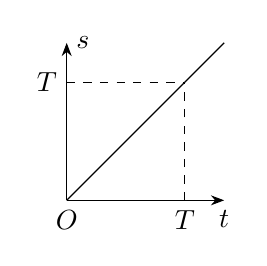
\begin{tikzpicture}[>=Stealth]
			\draw [->](0,0)--(2,0)node[below]{$t$};
			\draw [->](0,0)--(0,2)node[right]{$s$};
			\draw (0,0)node[below]{$O$}--(2,2);
			\draw [dashed](1.5,0)node[below]{$T$}--(1.5,1.5);
			\draw [dashed](0,1.5)node[left]{$T$}--(1.5,1.5);
		\end{tikzpicture}
	\end{minipage}
	\begin{minipage}{0.3\textwidth}
		由于$\E[X(t)X(s)]=\lambda^2 st+\lambda \min\{s,t\}$,所以下面的积分式也分为$s=t$轴两边考虑,由于对称性
	\end{minipage}
	\[\begin{split}
		\E(X_T) &= \E\left(\frac{1}{T}\int_{0}^{T}X(t)\d t\right) = \frac{1}{T}\int_{0}^{T}\E[X(t)]\d t\\
		&= \frac{1}{T}\int_{0}^{T}\lambda t\d t = \frac{\lambda T^2}{2}\\
		\E(X^2_T) &= \E\left(\frac{1}{T}\int_{0}^{T}X(t)\d t\right)^2 = \frac{1}{T^2}\E\left[\int_{0}^{T}X(t)\d t \int_{0}^{T}X(s)\d s \right]\\
		&= \frac{1}{T^2}\E\left[\iint_{[0,T]^2} X(t)X(s)\d t \d s \right]\\
		&= \frac{2}{T^2}\int_{0}^{T}\d t\int_{0}^{t}\E[X(t)X(s)]\d s\\
		&= \frac{2}{T^2}\int_{0}^{T}\d t\int_{0}^{t}\lambda^2 st+\lambda \min\{s,t\}\d s\\
		&= \frac{2}{T^2}\int_{0}^{T}\d t\int_{0}^{t}(\lambda^2 st + \lambda s)\d s\\
		&= \frac{1}{4}\lambda^2 T^2 + \frac{1}{3}\lambda T
	\end{split}\]
\end{solution}

\begin{definition}{}{}
    Poisson过程第$n-1$到第$n$次事件间的间隔时间记作$X_n,\,W_n=\sum_{i=1}^{n}X_i$
    \par $X_n,n=1,2,\dots $是均值为$\frac{1}{\lambda}$的独立同分布的\textcolor{red}{指数随机变量},$W_n$服从参数为$n,\lambda$的$\Gamma $分布
\end{definition}

\section{Poisson过程的推广}
\begin{definition}{非齐次Poisson过程}{}
    Poisson过程$N(t)$的强度$\lambda$与$t$有关.定义计数过程$\{N(t),t\geq 0\}$称为一个\index{非齐次Poisson过程}\textcolor{red}{非齐次Poisson过程}且具有\index{强度函数}\textcolor{red}{强度函数}$\lambda(t)$,若它满足以下四条
    \begin{enumerate}
        \item $N(0)=0$
        \item $\{N(t),t\geq 0\}$为独立增量过程,但\textcolor{red}{不是}平稳独立增量过程
        \item $\p [N(t+h)-N(t)\geq 1]=\lambda (t)h+o(h)$
        \item $\p [N(t+h)-N(t)\geq 2]=o(h)$
    \end{enumerate}
\end{definition}
\begin{remark}
    $\displaystyle \p [N(t+h)-N(t)=k]=\frac{\left(\int_{t}^{t+h}\lambda(u)\d u\right)^k\e ^{-\int_{t}^{t+h}\lambda(u)\d u}}{k!}\quad (k\geq 0)$
    相对于齐次Poisson过程就是把$\lambda t$换成$\displaystyle \int_{t}^{t+h}\lambda(u)\d u$即可。
    故当$\lambda(t)\equiv \lambda$时,该过程为Poisson过程
\end{remark}

\begin{definition}{复合Poisson过程}{}
    $\displaystyle X(t)=\sum_{i=1}^{\color{red} N(t)}Y_i\, (Y_i\, \iid)$ $X(t)$为\index{复合Poisson过程}\textcolor{red}{复合Poisson过程}($t\geq 0$,当$N(t)=0$,约定$X(t)=0$)
    \par $\color{red} N(t)$是强度为$\lambda$的Poisson过程,且$N(t)$与$\{Y_i,i\geq 1\}$独立(故$X(t)$即为随机和)
    \par 若$Y_i$的分布函数$G(y)$,且$\E [Y_i]=M, \quad \var (Y_i)=\sigma ^2$
    \begin{enumerate}
        \item 则有$\E [X(t)]=\E [N(t)]\E [Y_i]=\lambda \mu t$
        \item $\var (X(t))=\E [N(t)]\var (Y)+\var (N(t))\E ^2[Y]=\lambda (\mu ^2+\sigma ^2)t$
    \end{enumerate}
\end{definition}
\begin{remark}
    可以求$g_{X(t)}(v)$
    \[\begin{aligned}
        g_{X(t)}(v)&=\E [\e ^{vX(t)}]=\E [\E [\e ^{v\sum_{i=1}^{N(t)}Y_i}|N(t)]]=\E [g_Y^{N(t)}(v)]\\
        &=\sum_{n=0}^{\infty}g_Y^n(v)\p [N(t)=n]=\sum_{n=0}^{\infty}\frac{(\lambda tg_Y(0))^n}{n!}\e ^{-\lambda t}=\e ^{\lambda tg_Y(v)}\cdot \e ^{-\lambda t}\\
        &=\e ^{\lambda t(g_Y(v)-1)}
    \end{aligned}\]
\end{remark}

\begin{example}
    课本$\mathbf{P}_{21}$\textbf{例2.4}假定股票交易次数是以$\lambda$为速率的Poisson过程,记第$k$次与第$k-1$次交易前后股价变化为$Y_k$.不妨假定$Y_1,Y_2,\dots \iid$且与$N(t)$独立,$X(t)=\sum_{k=1}^{N(t)}Y_k$代表到时刻$t$时股票的总价格变化.设$Y_i$的分布为$G(y)$,试求$F_{X(t)}(x)=\p [X(t)\leq x]$
    \begin{solution}
        \[\p [Y_1+Y_2 \leq y]=\int_{-\infty}^{+\infty}G(y-z)\d G(z)\triangleq G*G(y)=G^{(2)}(y) \]
        由此递推,可定义
        \[G^{(n)}(y)=\underbrace{G*G*\cdots *G(y)}_{n\text{个}}=G^{(n-1)}*G(y)=\int_{-\infty}^{+\infty}G^{(n-1}(y-z)\d G(z)=\p [Y_1+Y_2+\cdots +Y_n\leq y]\]
        由此\[F_{X(t)}(x)=\p [X(t)\leq x]=\p [\sum_{k=1}^{N(t)}Y_k\leq x]=\E [I_{\sum_{k=1}^{N(t)Y_k\leq x}}]=\E [\E [I_{\sum_{k=1}^{N(t)}Y_k\leq x}|N(t)]]\]
        先求\[\E [I_{\sum_{k=1}^{N(t)}}|N(t)]=\E [I_{\sum_{k=1}^{n}Y_k\leq x}]=\p [\sum_{k=1}^{n}Y_k\leq x]=G^{(n)}(x)\]
        推得\[F_{X(t)}(x)=\E [G^{(N(t))}(x)]=\sum_{n=0}^{\infty}\frac{(\lambda t)^n\e ^{-\lambda t}}{n!}G^{(n)(x)}\]
    \end{solution}
\end{example}

\begin{remark}
    复合Poisson过程矩母函数推导:
    \begin{enumerate}
        \item 若$Y_i\equiv 1(i\geq 1),g_Y(v)=\E [\e ^{v}]=\e ^{v}\Rightarrow g_{X(t)}(v)=\e ^{\lambda t(\e ^{v}-1)}\Rightarrow X(t)\sim \text{Poisson}(\lambda t)$
        \item 若$Y_i\sim B(1,p)(i\geq 1)$,则$g_Y(v)=p\e ^{v}+1-p\Rightarrow g_{X(t)}(v)=\e ^{\lambda pt(\e ^{v}-1)}\Rightarrow X_(t)\sim \text{Poisson}(\lambda pt)$,此时$X(t)$是一个强度为$\lambda p$的Poisson过程(习题2.9)
    \end{enumerate}
\end{remark}

\begin{definition}{更新过程}{}
    Poisson过程的时间间隔为$X_i\sim Exp(\lambda )$,更新过程则是把$X_i$改为分布函数为$F(x)$的随机变量.
    记$W_0=0,\, W_n=\sum_{i=1}^{n}X_i$,$W_n$表示第$n$次事件发生的时刻,则称
    \[N(t)=\max {n:W_n\leq t}\]为\index{更新过程}\textcolor{red}{更新过程},$m(t)=\mu _N(t)=\E [N(t)]$为\index{更新函数}\textcolor{red}{更新函数}
\end{definition}

\section{习题}
\subsection{等待时间与时间间隔}
\begin{example}
    设$\{W_n\}$是与Poisson过程$N(t)$对应的一个等待时间序列(即$W_n$为第$n$个事件发生的时刻)
    \[\begin{aligned}
        \p [W_n\leq t]&=\p [N(t)\geq n]=\sum_{j=n}^{\infty}\frac{(\lambda t)^j\e ^{-\lambda t}}{j!}\\
        \textcolor{red}{f(t)}&=\frac{\mathrm{d}}{\mathrm{d}t}\left(\p [W_n\leq t]\right)=-\sum_{j=n}^{\infty}\frac{(\lambda t)^j}{j!}\lambda \e ^{-\lambda t}+\sum_{j=n}^{\infty}\lambda \e ^{-\lambda t}\frac{(\lambda t)^{j-1}}{(j-1)!}=\color{red}\lambda \e ^{-\lambda t}\frac{(\lambda t)^{n-1}}{(n-1)!}
    \end{aligned}\]
\end{example}
\begin{example}
    (课本$\mathbf{P}_{25}\mathbf{T}_{14}$),判断下述命题的真伪
    \begin{enumerate}
        \item $\{N(t)<k\}\Leftrightarrow \{W_k>t\}$
        \item $\{N(t)\leq k\}\Leftrightarrow \{W_k\geq t\}$
        \item $\{N(t)>k\}\Leftrightarrow \{W_k<t\}$
    \end{enumerate}
    \begin{solution}
        1.$\Leftrightarrow$\qquad 2.$\nrightarrow$且$\nleftarrow$\qquad 3.$\rightarrow \nleftarrow$
    \end{solution}
\end{example}
\begin{example}
    (课本$\mathbf{P}_{25}\mathbf{T}_{11}$)冲击模型(Shock Model)记$N(t)$为某系统到某时刻$t$受到的冲击次数,它是参数为$\lambda$的Poisson过程.设第$k$次冲击对系统的损害大小$Y_k$服从参数为$\mu$的指数分布,$Y_k,k=1,2,\dots ,\,\iid $.记$X(t)$为系统所受到的总损害.当损害超过一定的极限$\alpha$时系统寿命终止,记$T$为系统寿命,求$\E [T]$
    \par 提示:对非负随机变量$\displaystyle \E [T]=\int_{0}^{+\infty}\p [T>t]\d t$
    \begin{solution}\textcolor{red}{1}
        \[\begin{aligned}
            1-F_T(t)&=\p [T<t]=\p [X(t)<\alpha ]=\p \left[\sum_{k=1}^{N(t)}Y_k\leq \alpha \right]=\sum_{n=1}^{\infty}\p \left[\sum_{k=1}^{N(t)}Y_k\leq \alpha |N(t)=n\right]\p [N(t)=n]\\
            &=\sum_{n=1}^{\infty}\p [\sum_{k=1}^{n}Y_k\leq \alpha ]\p [N(t)=n]
        \end{aligned}\]
        $Y_1,Y_2,\dots ,Y_n\iid$且$Y_i\sim Exp(\mu )$.设$S_n=\sum_{k=1}^{n}Y_k$
        由独立同分布的指数分布随机和为参数为$(n,\mu)$的$\Gamma$分布
        \[f_{S_n}(s)=\mu \frac{\e ^{-\mu s}(\mu s)^{n-1}}{(n-1)!}\]
        \[\p [S_n\leq \alpha]=\int_{0}^{\alpha}\mu \frac{\e ^{-\mu s}(\mu s)^{n-1}}{(n-1)!}\d s=\frac{\mu}{(n-1)!}\int_{0}^{\alpha}\e ^{-\mu s}(\mu s)^{n-1}\d s\]
        \[\begin{aligned}
            1-F_T(t)&=\sum_{n=1}^{\infty}\frac{\e ^{-\lambda t}(\lambda t)^n}{n!}\cdot \frac{\mu}{(n-1)!}\int_{0}^{\alpha}\e ^{-\mu s}(\mu s)^{n-1}\d s\\
            &=\mu \e ^{-\lambda t}\sum_{n=1}^{\infty}\int_{0}^{\alpha}\frac{(\lambda t)^n}{n!(n-1)!}\e ^{-\mu s}(\mu s)^{n-1}\d s\\
            &\xlongequal{\text{交换求和和积分符号}}\mu \e ^{-\lambda t}\int_{0}^{\alpha}\sum_{n=0}^{\infty}\frac{(\lambda t)^{n+1}}{(n+1)!}\frac{(\mu s)^n\e ^{-\mu s}}{n!}\d s\\
        \end{aligned}\]
        因为$\displaystyle \sum_{n=0}^{\infty}\frac{(\lambda t)^{n+1}}{(n+1)!}=\e ^{\lambda t}-1 ,\quad \sum_{n=0}^{\infty}\frac{(\mu s)^n\e ^{-\mu s}}{n!}=1$
        \\ 所以由\textcolor{red}{Mertens定理}得$\displaystyle \sum_{n=0}^{\infty}\frac{(\lambda t)^{n+1}}{(n+1)!}\frac{(\mu s)^n\e ^{-\mu s}}{n!}=(\e ^{\lambda t}-1)\cdot 1=\e ^{\lambda t}-1$
        \[\begin{aligned}
            1-F_T(t)&=\mu \e ^{-\lambda t}\int_{0}^{\alpha}(\e ^{\lambda t}-1)\cdot 1\d s=\mu \alpha (1-\e ^{-\lambda t})\\
            f_T(t)&=-\frac{\mathrm{d}}{\mathrm{d}t}(1-F_T(t))=\lambda \mu \alpha \e ^{-\lambda t}\\
            \E [T]&=\int_{0}^{+\infty}tf_T(t)\d t=\frac{\mu \alpha}{\lambda }
        \end{aligned}\]
    \end{solution}
    \begin{solution}\textcolor{red}{2}
        可以采用不那么暴力的方法,即使用题目里的提示$\displaystyle \E [T]=\int_{0}^{+\infty}\p [T>t]\d t$,
        先把这个提示证一遍
        \[\begin{aligned}
            \int_{0}^{+\infty}\p [T>t]\d t &=\int_{0}^{+\infty}\left(\int_{t}^{+\infty}f_T(x)\d x\right)\d t\xlongequal{\text{交换积分次序}}\\
            &=\int_{0}^{+\infty}\d x \int_{0}^{x}f_T(x)\d t=\int_{0}^{+\infty}xf_T(x)\d x=\int_{0}^{+\infty}tf_T(t)\d t\\
            &=\E [T]
        \end{aligned}\]
        \[\begin{aligned}
            \p [T>t]&=1-F_T(t)=\mu \e ^{-\lambda t}\int_{0}^{\alpha}\sum_{n=0}^{\infty}\frac{(\lambda t)^{n+1}}{(n+1)!}\frac{(\mu s)^n\e ^{-\mu s}}{n!}\d s\\
            \E [T]&=\int_{0}^{+\infty}\p [T>t]\d t\\
            &=\sum_{n=1}^{\infty}\frac{(\mu \lambda)^n}{n!(n-1)!}\int_{0}^{+\infty}t^n\e ^{-\lambda t}\d t\cdot \int_{0}^{\alpha}s^{n-1}\e ^{-\mu s}\\
            &=\frac{1}{\lambda}\sum_{n=1}^{\infty}\frac{\mu ^n}{(n-1)!}\int_{0}^{\alpha}s^{n-1}\e ^{-\mu s}\d s\\
            &=\frac{1}{\lambda}\int_{0}^{\alpha}\e ^{-\mu s}\sum_{n=1}^{\infty}\frac{\mu ^n}{(n-1)!}s^{n-1}\d s\\
            &=\frac{\mu}{\lambda}\int_{0}^{\alpha}\d s=\frac{\mu \alpha}{\lambda}
        \end{aligned}\]
    \end{solution}
\end{example}
\begin{example}
    一部仪器受到的冲击数$N(t)$为强度$\lambda$的Poisson过程,设第$i$次冲击造成的损伤为$D_i,(i=1,2,\dots ,)\iid$并与$N(t)$独立。若损伤$D_i(t)=D_i\e ^{-\alpha t}(\alpha>0)$,则仪器所受的总损伤为
    \[D(t)=\sum_{i=1}^{N(t)}D_i\e ^{-\alpha (t-W_i)}\]
    其中$W_i$为第$i$次冲击来到的时刻,试求$\E [D(t)]$,假定$\E [D_i]=D$
    \begin{solution}
        \[\E \left[\left.\sum_{i=1}^{N(t)}D_i\e ^{-\alpha(t-W_i)}\right|N(t)=n\right]=D\e ^{-\alpha t}\sum_{i-1}^{n}\E \left[\left.\e ^{-\alpha W_i}\right|N(t)=n\right]\]
        {\color{red}由于求和把每个$W_i$都算上了,和次序无关,则$W_i\sim U(0,t)$,则\[\E [\e ^{-\alpha W_i}]=\frac{\e ^{\alpha t}-1}{\alpha t}\]}
        则\[\E \left[\sum_{i=1}^{N(t)}D_i\e ^{-\alpha(t-W_i)}\right]=\E \left[\E \left[\left.\sum_{i=1}^{N(t)}D_i\e ^{-\alpha(t-W_i)}\right|N(t)\right]\right]=\frac{\lambda D}{\alpha}(1-\e ^{\alpha t})\]
    \end{solution}
\end{example}

\chapter{Markov过程}
\section{Markov链的定义和例子}
\begin{definition}{Markov过程}{Markov Chain}
    设有随机过程(序列)$\{X_n,n=1,2,\dots \}\triangleq\{X_n,n>0\}$,其状态空间为有限集合(常表为$S=\{0,1,2\dots\}$)。
    \par 若对一系列状态$i_0,i_1,\dots ,i_n\in S$满足\index{马氏性}\textcolor{red}{马氏性}:
    \[\p [X_{n+1}=i_{n+1}|X_0=i_0,\dots ,X_n=i_n]=\p [X_{n+1}=i_{n+1}|X_n=i_n]\]
    则称$\{X_n,n\geq 0\}$为一个\index{Markov过程}\textcolor{red}{(离散时间)马尔可夫链(M.C.)}
\end{definition}

\begin{definition}{一步转移概率}{}
    $p_{ij}^{n,n+1}=\p [X_{n+1}=i_{n+1}|X_n=i_n]$称为Markov链的\index{一步转移概率}\textcolor{red}{一步转移概率}.若该概率与$n$无关时则称Markov链有\index{平稳转移概率}\textcolor{red}{平稳转移概率}(亦称为\index{时齐Markov链}\textcolor{red}{时齐Markov链}),并记为$p_{ij}$
    \[p_{ij}\geq 0\quad \sum_{j=0}^{\infty}p_{ij}=1(\text{这点很重要,意味着Markov链中不存在孤立的状态})\]
    把$p_{ij}$排成一个无穷维的方程,称为\index{转移概率矩阵}\textcolor{red}{转移概率矩阵},表示为
    \[\bm{P}=\begin{pmatrix}
      p_{00} & p_{01} & p_{02} & \cdots \\
      p_{10} & p_{11} & p_{12} & \cdots \\
       &  & \vdots &  \\
      p_{n0} & p_{n1} & p_{n2} & \cdots \\
       &  & \vdots & 
    \end{pmatrix}\]
\end{definition}

\begin{proposition}{}{}
    一个(时齐的)M.C.可由其初始分布及其一步转移概率完全确定。即若设$\p [X_0=i_0]=p_{i_0}$则对$\forall i_0,\dots ,i_n\in S$有
    \[\p [X_0=i_0,X_1=i_1,\dots ,X_n=i_n]=p_{i_0}p_{i_0i_1}p_{i_1i_2}\dots p_{i_{n-1}i_n}\]
    由条件概率公式\[\color{red}\p [BC|A]=\p [B|A]\p[C|AB]\]
    记$A_k\triangleq\{X_k=i_k\}$,可以推导
    \[\p[A_0A_1\dots A_n]=\p[A_0]\p[A_1|A_0]\p[A_2|A_0A_1]\dots \p[A_n|A_0A_1\dots A_{n-1}]\]
\end{proposition}

\begin{definition}{n步转移概率}{}
    $p_{ij}^{(n)}=\p [X_{m+n}|X_m=i]$称为Markov链的\index{$n$步转移概率}\textcolor{red}{$n$步转移概率}.有$n$步转移概率矩阵$\bm{P}^{(n)}=\bm{P}\times \bm{P}\times \cdots \bm{P}=\bm{P}^n$,这样导出下面的定理
\end{definition}
\begin{theorem}{Chapman-Kolmogorov}{Chapman-Kolmogorov}
    Markov链的$n$步转移概率矩阵满足\[p_{ij}^{(n)}=\sum_{k=0}^{\infty}p_{ik}p_{kj}^{(n-1)}\]
    约定$p_{ii}^{(0)}=1$,当$j\neq i$时,$p_{ij}^{(0)}=0$.\textcolor{red}{Chapman-Kolmogorov方程}(\index{C-K方程}C-K方程):
    \[\forall m,n\geq 0,\bm{P}^{(m+n)}=\bm{P}^{(n)}\times \bm{P}^{(m)}\]
    \[p_{ij}^{(n+m)}=\sum_{k=0}^{\infty}p_{ik}^{n}p_{kj}^{(m)}\]
    \begin{proof}
        \[\begin{aligned}
            p_{ij}^{(n)}&=\p[X_n=j|X_0=i]=\sum_{k=0}^{\infty}\p[X_n,X_1=k|X_0=i]\\
            &=\sum_{k=0}^{\infty}\p[X_1=k|X_0=i]\p[X_n=j|X_0=i,X_1=k]\\
            &\xlongequal{\text{\textcolor{red}{马氏性}}}\sum_{k=0}^{\infty}\p[X_1=k|X_0=i]\p[X_n=j|X_1=k]\\
            &=\sum_{k=0}^{\infty}p_{ik}p_{kj}^{(n-1)}
        \end{aligned}\]
    \end{proof}
\end{theorem}

\section{Markov链的状态分类}
\begin{definition}{可达与互达}{accessible communicate}
    若对某一$n\leq 0$,有$p_{ij}^{(n)}>0$,则称状态$j$是从状态$i$\index{可达的}\textcolor{red}{可达的}(accessible),记作$i\rightarrow j$.表示从$i$经过\textcolor{red}{有限步}的转移可以到达$j$.
    两个互相可达的状态$i,j$则称为\index{互达的}\textcolor{red}{互达的}(communicate)
    \par 互达性是一种等价关系,满足自反性、对称性和传递性.
    若两个状态互达则称为在同一等价类中,Markov链因此被分割为不同等价类的无交并.
    \par 若一个Markov链是所有状态处于同一等价类,则称之是\index{不可约的}\textcolor{red}{不可约的}(irreducible).
\end{definition}
\begin{remark}
    证明传递性:$i\leftrightarrow j,j\leftrightarrow k \Rightarrow i\leftrightarrow k$\quad 假设$p_{ij}^{(n)}>0,p_{jk}^{(m)}>0$
    \[p_{ik}^{(n+m)}\xlongequal{\text{C-K方程}}\sum_{r=0}^{\infty}p_{ir}^{(n)}p_{rk}^{(m)}\geq p_{ij}^{(n)}p_{jk}^{(m)}>0\]
\end{remark}
\begin{note}
    \begin{enumerate}
        \item M.C.的所有状态由“互达”关系可分为若干不同的等价类的并集.
              \[S=S_1\oplus S_2\oplus \cdots \oplus S_k\oplus \cdots \]
              每个等价类内的任意两个状态皆互达,分属不同等价类的两个状态必不互达,不同等价类之间不相交
        \item 马氏链称为不可约的当且仅当其所有状态处于同一等价类中
        \item 闭集:状态空间$S$的子集$S'\subseteq S$称为M.C.的闭集若它满足:对于$\forall i\in S'$并且$i\to j$,则必可推出$j\in S'$.显然,最大的闭集即为$S$本身.“极小闭集”$A$若$A$的任意真子集不再是闭集.
              \par 马氏链$\{X_n,n\geq 0\}$限制在其闭集$S'$上仍为一马氏链,且转移概率矩阵$\bm{P'}=(p_{ij})_{i,j\in S'}$.只有一个状态的闭集即为\textcolor{red}{吸收态},故闭集可认为是吸收态的推广.
    \end{enumerate}
\end{note}

\begin{example}
    \textbf{例3.6}($\mathbf{P}_{32}$)设Markov链的转移概率矩阵为:
    \[\bm{P}=\bordermatrix{
        & 1 & 2 & 3 & 4 & 5 \cr
      1 & \frac{1}{4} & \frac{3}{4} & 0 & 0 & 0 \cr
      2 & \frac{1}{2} & \frac{1}{2} & 0 & 0 & 0 \cr
      3 & 0 & 0 & 0 & 1 & 0 \cr
      4 & 0 & 0 & \frac{1}{2} & 0 & \frac{1}{2} \cr
      5 & 0 & 0 & 0 & 1 & 0}
    =\begin{pmatrix}
      \bm{A} & \bm{O} \\
      \bm{O} & \bm{B} \\
    \end{pmatrix}\]
    试讨论其状态分类
    \begin{solution}
        由于$\bm{P}^{(n)}=\bm{P}^n=\begin{pmatrix}  \bm{A}^n & \bm{O} \\  \bm{O} & \bm{B}^n\end{pmatrix}$故若状态分属于$S_1=\{1,2\},S_2=\{3,4,5\}$,则必有$p_{ij}^{(n)}\equiv 0\,(\forall n\geq 0)$,从而$S_1,S_2$不在同一个等价类中
        \par 又因1,2显然互达,即$S_1$中两状态互达。$S_2$中状态也是互达的,于是$S=S_1 \oplus S_2$
        状态转移图如下
        \begin{center}
            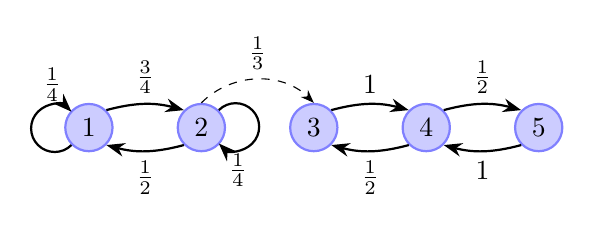
\begin{tikzpicture}
                [%%%%%%%%%%%%%%%%%%%%%%%%%%%%%%%%%%%%%%%%%%%%%%%%%%%%%%%%%%
                    node distance =.8cm,>=Stealth,
                    place/.style={circle,draw=blue!50,fill=blue!20,thick,
                                  inner sep=0pt,minimum size=6mm}
                ]%%%%%%%%%%%%%%%%%%%%%%%%%%%%%%%%%%%%%%%%%%%%%%%%%%%%%%%%%%
                \node[place] (1) {$1$};
                \node[place] (2) [right=of 1] {$2$};
                \node[place] (3) [right=of 2] {$3$};
                \node[place] (4) [right=of 3] {$4$};
                \node[place] (5) [right=of 4] {$5$};

                \draw [->,thick] (1.south west) arc (-45:-315:0.3) node [above left] {$\frac{1}{4}$};
                \draw [->,thick] (2.north east) arc (135:-135:0.3) node [below right] {$\frac{1}{4}$};
                \draw [->,thick] (1.north east) to [bend left=15]  node[above] {$\frac{3}{4}$}  (2.north west);
                \draw [<-,thick] (1.south east) to [bend right=15]  node[below] {$\frac{1}{2}$}(2.south west);
                \draw [->,thick] (3.north east) to [bend left=15]  node[above] {1}  (4.north west);
                \draw [<-,thick] (3.south east) to [bend right=15]  node[below] {$\frac{1}{2}$}(4.south west);
                \draw [->,thick] (4.north east) to [bend left=15]  node[above] {$\frac{1}{2}$}  (5.north west);
                \draw [<-,thick] (4.south east) to [bend right=15]  node[below] {1}(5.south west);
                \draw [->,dashed] (2.north) to [bend left=45] node[above] {$\frac{1}{3}$} (3.north);
            \end{tikzpicture}
        \end{center}
        由图可见,该Markov链是把两个不互达的M.C.拼接在了一起,易见$S_1$和$S_2$是两个闭集,且均为极小闭集.其转移概率矩阵分别为$\bm{A},\bm{B}$,即使在图中再加一条转移途径(虚线),结论$S=S_1\oplus S_2$仍然为真.但此时$S_1$已经不再是闭集,其对应的子矩阵$\begin{pmatrix}  \frac{1}{4} & \frac{3}{4} \\ \frac{1}{3} & \frac{1}{3} \end{pmatrix}$也不再是随机矩阵,但$S_2$仍为(极小)闭集。
    \end{solution}
\end{example}

\begin{definition}{\index{Markov周期性}Markov周期性}{}
    使得$p_{ii}^{(n)}>0$的所有正整数$n(n\geq 1)$的\textcolor{red}{最大公约数}称为$i$的周期,记为$d(i)$.
    \par 若$\forall n\in \mathbb{N}^* ,p_{ii}^{(n)}=0$则约定周期为$\infty$.
    \par $d(i)=1$的状态则称为是\textcolor{red}{非周期的},由定义得,若$d(i)\nmid n$,则$p_{ii}^{(n)}=0$
\end{definition}
\begin{note}
    这是一个奇怪的定义.我们参考下面这个例子.
\end{note}
\begin{example}课本$\mathbf{P}_{33}$\textbf{例3.7}
    \begin{center}
        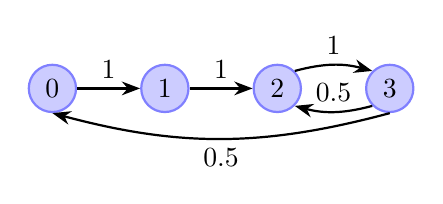
\begin{tikzpicture}
            [%%%%%%%%%%%%%%%%%%%%%%%%%%%%%%%%%%%%%%%%%%%%%%%%%%%%%%%%%%
                node distance =.8cm,>=Stealth,
                place/.style={circle,draw=blue!50,fill=blue!20,thick,
                              inner sep=0pt,minimum size=6mm}
            ]%%%%%%%%%%%%%%%%%%%%%%%%%%%%%%%%%%%%%%%%%%%%%%%%%%%%%%%%%%
            \node[place] (0) {$0$};
            \node[place] (1) [right=of 0] {$1$};
            \node[place] (2) [right=of 1] {$2$};
            \node[place] (3) [right=of 2] {$3$};
        
            \draw [->,thick] (0.east) to node[above] {1}  (1.west);
            \draw [->,thick] (1.east) to node[above] {1}  (2.west);
            \draw [->,thick] (2.north east) to [bend left=15]  node[above] {1}  (3.north west);
            \draw [<-,thick] (2.south east) to [bend right=15]  node[above] {0.5}(3.south west);
            \draw [->,thick] (3.south) to [bend left=15] node[below] {0.5} (0.south);
        \end{tikzpicture}
    \end{center}
    易得使$p_{00}^{(n)}>0$成立的$n=4+2k,d(0)=\mathrm{gcd}(4,6,8,\dots)=2$
\end{example}
\begin{proposition}{等价类的周期}{}
    若$i\leftrightarrow j$,则$d(i)=d(j)$
    \begin{proof}
        由$i\leftrightarrow j$得$\exists m,n,s.t.p_{ij}^{(m)}>0,p_{ji}^{(n)}>0$
        则有\[p_{jj}^{(n+m)}\geq p_{ji}^{(n)}p_{ij}^{(m)}>0\]
        假如有$s, s.t.p_{ii}^{(s)}>0$
        则也有\[p_{jj}^{(n+s+m)}\geq p_{ji}^{(n)}p_{ii}^{(s)}p_{ij}^{(m)}>0\]
        所以$d(j)|n+m\quad d(j)|n+s+m\Rightarrow d(j)|s$又$d(i)|s\Rightarrow d(j)|d(i)$同理$d(i)|d(j)\Rightarrow d(i)=d(j)$
    \end{proof}
    \color{red}故一个互达等价类中的每个状态的周期相等.
\end{proposition}
\begin{proposition}{}{}
    若状态$i$有周期$d(i)$,则存在整数$N$,使得$\forall n>N,p_{ii}^{(nd(i))}>0$,证明需要用数论,略
\end{proposition}

\begin{corollary}{}{}
    若$p_{ji}^{(m)}>0$, 则$\exists N\in \mathbb{N}^* ,s.t. \forall n>N :P_{ji}^{(m+d(i))}>0$
\end{corollary}

\begin{proposition}{}{}
    令$\bm{P}$为\textcolor{red}{不可约,非周期,有限状态}Markov链的转移概率矩阵,则$\exists N\in \mathbb{N}^*$使得当$n\geq N$时,$\bm{P}^{(n)}$的\textcolor{red}{所有元素}都非零
\end{proposition}

\subsection{常返与瞬过}
\begin{definition}{\index{首次到达概率}首次到达概率}{}
    定义$f_{ij}^{(0)}$为从$i$出发在第$n$步\textcolor{red}{首次}到达$j$的概率(注意与$p_{ij}^{(n)}$的区别),即
    \[f_{ij}^{(n)}=\p [X_n=j,\textcolor{red}{X_k\neq j,k=1,\dots ,n-1}|X_n=i]\]
    约定$f_{ii}^{(0)}=f_{ij}^{(0)}=0$.
    \par 定义$f_{ij}=\sum_{n=1}^{\infty}f_{ij}^{(n)}$,表示从$i$出发\textcolor{red}{最终}转入状态$j$的概率.
    若$i\neq j$则$i\rightarrow j \Leftrightarrow f_{ij}>0$,直观看来,就是若$i$可达$j$则经过无穷步之后必然到达$j$,其和$p_{ij}^{(n)}$有以下大小关系
    \[P_{ij}^{(n)}=\p[X_n=j|X_0=i]\leq \p[\bigcup_{n=1}^{\infty}(X_n=j|X_0=i)]=f_{ij}\]
\end{definition}
\begin{definition}{常返(recurrent)与瞬过(transient)}{recurrent and transient}
    若$f_{ii}=1$则$i$是\index{常返}常返的,否则为\index{瞬过}瞬过的.
    \[f_{ii}=0\Leftrightarrow f_{ii}^{(n)}\equiv 0 \Leftrightarrow p_{ii}^{(n)}\equiv 0\Leftrightarrow d(i)=\infty\]
\end{definition}

\begin{theorem}{常返状态判断条件}{}
    \begin{enumerate}
        \item $i$常返$\Leftrightarrow \sum_{n=1}^{\infty}P_{ii}^{(n)}=\infty$(过程返回到$i$无穷多次)
        \item $i$瞬过$\Leftrightarrow \sum_{n=1}^{\infty}P_{ii}^{(n)}<\infty$(过程返回到$i$有限多次)
    \end{enumerate}
    $P_{ii}^{(n)}$是从$i$经过$n$步后到达$j$,中间可以已经到达过$j$,所以比$f_{ij}^{(n)}$缺少一个限制条件“首次”,故$P_{ij}^{(n)}\geq f_{ij}^{(n)}$
\end{theorem}
\begin{remark}
    设$\xi =\sum_{n=1}^{\infty}I_n =\sum_{n=1}^{\infty}I_{(X_n=i)}$,则$\xi$为整个过程中转移到$i$的次数,而\[\E[\xi|X_0=i]=\sum_{n=1}^{\infty}\E[I_{(X_n=i)}|X_0=i]=\sum_{n=1}^{\infty}\p[X_n=i|X_0=i]=\sum_{n=1}^{\infty}P_{ii}^{(n)}\]
    即为由$i$出发返回到$i$的平均次数,显然有$\color{red}\p[\xi \geq 1|X_0=i]=f_{ii}$,故有
    \[\p[\xi \geq 2|X_0=i]=\sum_{n=1}^{\infty}f_{ii}^{(n)}f_{ii}=f_{ii}\sum_{n=1}^{\infty}f_{ii}^{(n)}=f_{ii}^2\]
    且\textcolor{red}{一般有}\[\p[\xi \geq n|X_0=i]=f_{ii}^{(n)}\]
\end{remark}

\begin{corollary}{}{}
    若$i$是常返的,且$i\leftrightarrow j$,则$j$也是常返的.故处于同一互达等价类的状态具有相同的常返性
\end{corollary}
\begin{definition}{常返时}{}
    对常返状态$i$,定义$T_i$为首次返回状态$i$的时刻,称作\index{常返时}\textcolor{red}{常返时},记$\mu _i=\E [T_i]$(即平均常返时)
    \[\mu _i=\E[T_i|X_0=i]=\sum_{n=1}^{\infty}n\p[T_i=n|X_0=i]=\sum_{n=1}^{\infty}nf_{ii}^{(n)}\]
    有以下常返状态的分类:
    \begin{enumerate}
        \item 若$\mu _i=\infty$称$i$为\index{零常返}\textcolor{red}{零常返}
        \item 若$\mu _i<\infty$称$i$为\index{正常返}\textcolor{red}{正常返}
    \end{enumerate}
    不存在某常返态的平均常返时$\mu _i=0$,因为此时会推出$f_{ii}=0$,从而其为非常返
\end{definition}
\begin{remark}
    直观来看,\textcolor{red}{有限多个}状态的M.C.的$\mu _i$应该都有限的,而$\mu _i=+\infty$可能发生在\textcolor{red}{无穷多个}的Markov链的场合(例如直线上的简单对称随机游动)
\end{remark}
\begin{proposition}{}{}
    对于一个有限状态的Markov链,有以下性质
    \begin{enumerate}
        \item 它至少有一个状态是常返的
        \item 其任何常返状态必为正常返
    \end{enumerate}
\end{proposition}

\section{Markov链的极限定理与平稳分布}
\begin{theorem}{Markov链的基本极限定理}{}
    \begin{enumerate}
        \item 若状态$i$是\textcolor{red}{瞬过}的或者是\textcolor{red}{零常返}的,则\[\lim_{n \to \infty}P_{ii}^{(n)}=0\]
        \item 若状态$i$是\textcolor{red}{周期}为$d$的\textcolor{red}{常返}状态(零常返和正常返都对),则\[\lim_{n \to \infty}P_{ii}^{(n)}=\frac{d}{\mu _i}\]
        \item 若状态$i$是\textcolor{red}{非周期}的\textcolor{red}{正常返}(即\textcolor{red}{遍历态})状态,则\[\lim_{n \to \infty}P_{ii}^{(n)}=\frac{1}{\mu _i}\]
    \end{enumerate}
\end{theorem}
\begin{corollary}{}{}
    若$i$为遍历态,则对所有的$j\leftrightarrow i$有\[\lim_{n \to \infty}p_{ij}^{(n)}=\lim_{n \to \infty}p_{ii}^{(n)}=\frac{1}{\mu _i}\]
    这条推论有点反直觉
\end{corollary}
\begin{definition}{遍历性}{}
    一个\textcolor{red}{正常返}、\textcolor{red}{非周期}的状态也称作是\index{遍历}\textcolor{red}{遍历的}(ergodic),对遍历状态$i$有
    \[\lim_{n \to \infty}P_{ii}^{(n)}=\frac{1}{\mu _i}\]
\end{definition}

\begin{definition}{平稳分布}{}
    若Markov链有转移概率矩阵$\bm{P}=(P_{ij})$,且有一个概率分布
    \[\bm{\pi}=\{\pi_0,\pi_1,\dots ,\pi _j,\dots \}=\{\pi _i,i\geq 0\}\]若满足$\pi _j=\sum_{i=0}^{\infty}\pi _iP_{ij}$即$\bm{\pi }=\bm{\pi }\bm{P}$
    \[(\pi_0,\pi_1,\dots ,\pi _j,\dots )=(\pi_0,\pi_1,\dots ,\pi _j,\dots )\begin{pmatrix}
      p_{00} & p_{01} & \dots & p_{0j} & \dots \\
      p_{10} & p_{11} & \dots & p_{1j} & \dots \\
      \vdots & \vdots & \dots & \vdots & \vdots \\
      p_{j0} & p_{j1} & \dots & p_{jj} & \dots \\
      \vdots & \vdots & \dots & \vdots & \vdots \\
    \end{pmatrix}\]
    则称之为Markov链的\index{平稳分布}\textcolor{red}{平稳分布}
\end{definition}
\begin{remark}
    \begin{enumerate}
        \item 若$\bm{\pi }$为M.C.的一个平稳分布则$\displaystyle \bm{\pi }\mathbf{1}=1$,其中$\displaystyle \mathbf{1}=(1,1,\dots ,1,\dots )^T$
				\item 若$\bm{\pi }=\{\pi _j,j\geq 0\}$为Markov链的平稳分布,则还应该满足\[\pi _j=\sum_{i=0}^{\infty}\pi _ip_{ij}^{(n)}\qquad (j=0,1,2,\dots ,\quad n\in \mathbb{N}^*)\]
              即$\bm{\pi }=\bm{\pi }\bm{P}^{(n)}=\bm{\pi }\bm{P}^n$
        \item 若Markov链的初始分布$\bm{\pi }(0)$即为其平稳分布,则可推出:该Markov链为\textcolor{red}{严格平稳}过程
              \par 事实上,$\forall n\in \mathbb{N}$有\[\p[X_n=j]=\sum_{i=0}^{\infty}\p[X_0=i]=\p[X_n=j|X_0=i]=\sum_{i=0}^{\infty}\pi _iP_{ij}^{(n)}=\pi _j=\p[X_0=j]\]
              进一步,由马氏性和时齐性可得$\forall n,k\geq 0:(X_n,X_{n+1},\dots ,X_{n+k})\xlongequal{d}(X_0,X_1,\dots ,X_k)$(有限维分布平稳),从而$\{X_n,n\geq 0\}$为严平稳
    \end{enumerate}
\end{remark}

\begin{theorem}{平稳分布}{}
    若一个\textcolor{red}{不可约}Markov链中的所有状态都是\textcolor{red}{遍历}的,则对所有$i,j$有极限
    \[\lim_{n \to \infty}P_{ij}^{(n)}=\pi _j=\frac{1}{\mu _j}\qquad (\forall i,j=0,1,2,\dots )\]且存在$\sum_{j=0}^{\infty}\pi _j=1,\pi _j>0$
    \par 或者:一个\textcolor{red}{不可约、遍历}的Markov链比存在\textcolor{red}{唯一的}平稳分布$\bm{\pi }$,且即为该Markov链的极限分布
\end{theorem}

\begin{note}
    关于Markov链平稳分布的补充结论(免证)
    \begin{enumerate}
        \item Markov链存在平稳分布的\textcolor{red}{充要条件}是\textcolor{red}{存在正常返}状态
        \item \textcolor{red}{有限状态}的Markov链恒存在平稳分布
        \item \textcolor{red}{不可约}Markov链存在平稳分布的\textcolor{red}{充要条件}是方程组\[\pi _j=\sum_{i=0}^{\infty}\pi _iP_{ij}\qquad (j=0,1,2,\dots )\]
              有\textcolor{red}{非零的绝对收敛解},且此时方程组有\textcolor{red}{唯一的}绝对收敛解,即为平稳分布$\{\frac{1}{\mu _j},j\geq 0\}$
        \item \textcolor{red}{不可约有限状态}必有唯一的平稳分布
        \item \textcolor{red}{不可约遍历的}很有唯一的平稳分布且为极限分布$\pi _j=\lim_{n \to \infty}P_{ij}^{(n)}=\frac{1}{\mu _j}$
    \end{enumerate}
\end{note}

\section{分支过程(略)}
\begin{definition}{分支过程}{}
    刻画生物繁衍后代,物种遗传及原子核连锁反应等的数学模型,是一种特殊的Markov链.
    \par 分支过程(随机和):\[X_{n+1}=\sum_{i=1}^{X_n}Z_i^{(n)}\quad (N\geq 0)\]
    其中$X_0=1$(祖先).$Z_i^{(n)}$为第$n$代的第$i$个个体的子代个数.假定$Z_i^{(n)}(n\geq 0,i\geq 1)\iid $.$X_n$为第$n$代个体总数(不包括亲代)($X_0=1,X_1=Z_1^{(0)}$)
    \par 则$\{X_n,n\geq 0\}$为Markov链.群体消亡概率即吸收概率,但吸收概率求法与前几节不同,而是要利用离散型随机变量的\textcolor{red}{生成函数}的性质.
\end{definition}

\section{连续时间Markov链}
\begin{definition}{连续时间Markov链}{}
    设随机过程$\{X(t),t\geq 0 \}$的状态离散$S=\{0,1,2,\dots\}$,时间参数连续$T=[0,\infty)$.若$\forall s,t\geq 0 ,i,j\in S.x(u)\, (0\leq u<s)$满足:
    \[\p[X(s+t)=j|X(s)=i,X(u)=x(u),0\leq u<s]=\p[X(s+t)=j|X(s)=i]\]
    则称$\{X(t),t\geq 0\}$为一\index{连续时间Markov链}\textcolor{red}{连续时间Markov链}
    \par 并等价于以下定义:$\forall i_k\in S,\quad  0\leq t_0<t_1<t_2<\dots <t_n<t_{n+1}$
    \[\p[X(t_{n+1}=i_{n+1}|X(t_0)=i_0,X(t_1)=i_1,\dots ,X(t_n)=i_n]=\p[X(t_{n+1})=i_{n+1}|X(t_n)=i_n]\]
    若转移概率$\p[X(s+t)=j|X(s)=i]$与时刻$s$无关而仅与时间间隔$t$有关,则称$\{X(t),t\geq 0\}$具有\textcolor{red}{平稳的转移概率},并称此时的$X(t),t\geq 0$为时齐Markov链.
    \par 平稳转移概率记为\[\p[X(s+t)=j|X(s)=i]=\p[X(t)=j|X(0)=i\triangleq P_{ij}(t)]\]
    $P_{ij}(t)$又称为\index{转移概率函数}\textcolor{red}{转移概率函数}.$P_{ij}(t)$与$P_{ij}^{(n)}$的比较:$n \to t$
\end{definition}

\begin{theorem}{无瞬即转移}{}
    函数族$P_{ij}(t)$为一\index{无瞬即转移}\textcolor{red}{无瞬即转移}的充要条件为以下条件同时满足:
    \begin{enumerate}
        \item $\forall t\geq 0$,有\[P_{ij}(t)\geq 0,\sum_{j}P_{ij}(t)=\sum_{j=0}^{\infty}P_{ij}(t)=1\qquad (\forall i,j=0,1,2,\dots )\]
              即$\bm{P}(t)=\left(P_{ij}(t)\right)$为一随机矩阵
        \item 连续形式的C-K方程:\[P_{ij}(t+\tau )=\sum_{k=0}^{\infty}P_{ik}(t)P_{kj}(\tau)\]
              或者:\[P(t+\tau)=P(t)P(\tau)=P(\tau)=P(t)\]
        \item 无瞬即转移性:\[\forall i\in S:\lim_{\tau \to 0^+}\p[X(t+\tau)=i|X(t)=i]\xlongequal{\text{时齐}}\lim_{\tau \to 0}P_{ii}(\tau)=1\]
              进一步可写为\[\lim_{\tau \to 0^+}P_{ij}(\tau)=\lim_{\tau \to 0^+}\p[X(t+\tau )=j|X(t)=i]=\delta _{ij}=\begin{cases}
                1,&(j=i)\\
                0,&(j\neq i)
              \end{cases}=P_{ij}(0)\]
    \end{enumerate}
\end{theorem}
\begin{note}
    \begin{enumerate}
        \item 无瞬即转移性:过程转到状态$i$后悔停留一段时间,不会瞬即离去。满足该性质的Markov链称为\index{标准的Markov链}\textcolor{red}{标准的M.C.}
        \item 设$\tau _i$表示在状态$i$上的停留时间(r.v.),则由过程的马氏性得
              \[\forall s,t\geq 0:\p[\tau _i<s+t|\tau _i>s]=\p[\tau _i>t]\]
              此时称$\tau _i$有\textcolor{red}{无记忆性}.$\tau _i\sim Exp(\nu_i)$.且$\E[\tau _i]=\frac{1}{\nu _i}$,$\nu _i$可视为过程离开$i$的速率。
              \par $\nu _i=0$(吸收态) $\nu _i=+\infty$(瞬即转移)
        \item 定义$P_{ij}$为过程离开$i$转移到$j$的概率,则$\sum_{j\neq i}P_{ij}=1$.定义$q_{ij}=\nu _iP_{ij}$,称之为过程从$i$到$j$的转移率,显然$\sum_{j\neq i}q_{ij}=\nu _i$
    \end{enumerate}
\end{note}

\section{Markov链总结}
\begin{figure}[H]
	\centering
	\begin{tikzpicture}[>=Stealth]
		\path (0,0) node (node1) [shape=rectangle,draw,fill=pink!50] {$\{n|n\geq 1,p_{ii}^{(n)}>0\}\begin{cases}\text{空集,周期无穷大}\\ \text{非空}\begin{cases}d=1,\text{非周期的}\\ d>1,\text{周期的}\end{cases}\end{cases}$}
					(0,-2) node (node2) [shape=rectangle,draw,fill=red!20] {状态$i$}
					(0,-3.5) node [shape=rectangle,draw] {$\displaystyle \sum_{n=0}^{\infty}p_{ii}^{(n)}=\frac{1}{1-f_{ii}}$}
					(-3.5,-3.5) node {$\displaystyle f_{ii}=1\text{或}\sum_{n=0}^{\infty}p_{ii}^{(n)}=\infty$}
					(3.5,-3.5) node {$\displaystyle f_{ii}<1\text{或}\sum_{n=0}^{\infty}p_{ii}^{(n)}<\infty$}
					(-1.65,-5) node (node3) [shape=rectangle,draw,fill=green!20] {常返态$i$}
					(1.65,-5) node (node4) [shape=rectangle,draw,fill=gray!20] {非常返态$i$(瞬过)}
					(-3.7,-5) node {类性质}
					(-3.7,-6) node (left1) {$\text{若}i\leftrightarrow j\Rightarrow f_{ij}=1$}
					(-4.3,-7) node (left2) {$\displaystyle \text{周期为}d,\lim_{n \to \infty}p_{ii}^{(nd)}=\frac{d}{\mu_i}$}
					(-1.65,-8.5) node [shape=rectangle,draw] {$\displaystyle \mu_i=\sum_{n=1}^{\infty}nf_{ii}^{(n)}$}
					(-4,-8.5) node {$\mu_i<+\infty$}
					(0.7,-8.5) node {$\mu_i=+\infty$}
					(-3.1,-10) node (ll1) [shape=rectangle,draw,fill=yellow!20] {正常返$i$}
					(-0.2,-10) node (lr1) [shape=rectangle,draw,fill=blue!20] {零常返$i$}
					(-5,-11) node (ll2) {$\displaystyle \lim_{n \to \infty}p_{ii}^{(nd)}=\frac{d}{\mu_i}$}
					(-6,-12) node (ll3) {$\displaystyle \forall j\leftrightarrow i,j\in \mathcal{S},\lim_{n \to \infty}p_{ji}^{(n)}=\frac{d}{\mu_i}$}
					(-6.3,-13) node (ll4) {$\displaystyle \forall j\leftrightarrow i,j\in \mathcal{S},\lim_{n \to \infty}\frac{1}{n}\sum_{k=1}^{n}p_{ji}^{(k)}=\frac{d}{\mu_i}$}
					(-2.9,-13.8) node {非周期的$\Longleftrightarrow d(i)=1$}
					(-3.1,-14.6) node (ll5) [shape=rectangle,draw,fill=brown!20] {遍历态$i$}
					(-3.7,-15.4) node {$f_{ii}^{(1)}=1$}
					(-3.1,-16.2) node (ll6) [shape=rectangle,draw,fill=brown!20] {吸收态$i$}
					(1.9,-11) node (lr2) {$\displaystyle \lim_{n \to \infty}p_{ii}^{(nd)}=\frac{d}{\mu_i}=0$}
					(1.9,-12) node (lr3) {$\displaystyle \lim_{n \to \infty}p_{ii}^{(n)}=0$}
					(2.5,-13) node (lr4) {$\displaystyle \forall j\leftrightarrow i,j\in \mathcal{S},\lim_{n \to \infty}p_{ji}^{(n)}=0$}
					(2.5,-14) node (lr5) {$\displaystyle \forall j\leftrightarrow i,j\in \mathcal{S}, \lim_{n \to \infty}\frac{1}{n}\sum_{k=1}^{n}p_{ji}^{(k)}=0$};
		\draw [dashed](-2.8,-4.5) rectangle (3.5,-5.5);
		\draw [dashed](-4,-9.5) rectangle (0.9,-10.5);
		\draw [->] (node1) to (node2);
		\draw [->,rounded corners=10pt] (node2)--(0,-2.6) -- (-1.65,-2.6) to (node3);
		\draw [->,rounded corners=10pt] (node2)--(0,-2.6) -- (1.65,-2.6) to (node4);
		\draw [->,rounded corners=10pt] (node3)--(-1.65,-6) to (left1);
		\draw [->,rounded corners=10pt] (node3)--(-1.65,-7) to (left2);
		\draw [->,rounded corners=10pt] (node3)--(-1.65,-7.7)--(-3.1,-7.7) to (ll1);
		\draw [->,rounded corners=10pt] (node3)--(-1.65,-7.7)--(-0.2,-7.7) to (lr1);
		\draw [->,rounded corners=10pt] (ll1)--(-3.1,-11) to (ll2);
		\draw [->,rounded corners=10pt] (ll1)--(-3.1,-12) to (ll3);
		\draw [->,rounded corners=10pt] (ll1)--(-3.1,-13) to (ll4);
		\draw [->,rounded corners=10pt] (ll1)to (ll5);
		\draw [->,rounded corners=10pt] (ll5)to (ll6);
		\draw [->,rounded corners=10pt] (lr1)--(-0.2,-11) to (lr2);
		\draw [->,rounded corners=10pt] (lr1)--(-0.2,-12) to (lr3);
		\draw [->,rounded corners=10pt] (lr1)--(-0.2,-13) to (lr4);
		\draw [->,rounded corners=10pt] (lr1)--(-0.2,-14) to (lr5);
		\draw [->,rounded corners=10pt] (node4)--(4.3,-5)--(4.3,-11) to (lr2);
		\draw [->,rounded corners=10pt] (node4)--(4.3,-5)--(4.3,-12) to (lr3);
		\draw [->,rounded corners=10pt] (node4)--(5.3,-5)--(5.3,-13) to (lr4);
		\draw [->,rounded corners=10pt] (node4)--(5.6,-5)--(5.6,-14) to (lr5);
	\end{tikzpicture}
\end{figure}
\begin{figure}[H]
	\centering
	\begin{tikzpicture}[>=Stealth]
		\path (0,0) node (node1) {有一个零常返状态,则有无限个 零常返状态}
					(0,-2) node (node2) [shape=rectangle,draw,fill=red!20] {Markov链}
					(-3.7,-1) node (left1) [shape=rectangle,draw,fill=blue!20] {非时齐Markov链}
					(-4,-2) node {转移概率$p_{ij}$是否只与$i,j$有关}
					(-3.7,-3) node (left2) [shape=rectangle,draw,fill=green!20] {时齐的Markov链}
					(4.0,-1) node (right1) [shape=rectangle,draw,fill=orange!20] {无限链}
					(3.5,-2) node {状态是否有限}
					(4.0,-3) node (right2) [shape=rectangle,draw,fill=gray!20] {有限链}
					(-3.7,-4) node {所有状态互通$\Longleftrightarrow$ 只有1个类}
					(-1,-5) node (left3) [shape=rectangle,draw,fill=green!20] {不可约的}
					(0.7,-4) node {多于1个类}
					(1,-5) node (right3) [shape=rectangle,draw,fill=brown!20] {可约的}
					(-5,-6) node {所有状态遍历}
					(4,-4) node (text1) {不可能全为非常返}
					(4.15,-5) node (text2) {不可能有零常返}
					(-1,-6) node {所有状态非周期}
					(-1,-7) node (left4) [shape=rectangle,draw,fill=yellow!20] {不可约非周期的Markov链}
					(-3,-8) node {所有状态正常返}
					(1.8,-8) node{所有状态非常返或零常返}
					(3,-9) node (text3) {平稳分布不存在}
					(-5,-10) node (left5) [shape=rectangle,draw,fill=purple!20] {遍历的Markov链}
					(6,-7) node {只能是}
					(6,-8) node (right4) [shape=rectangle,draw,fill=blue!20]{正常返的Markov链}
					(1,-9.7) node {所有状态非周期($d=1$)}
					(-2,-11) node (text4) {$\displaystyle \lim_{n \to \infty}p_{ij}^{(n)}=\pi_j=\frac{d}{\mu_i}=\frac{1}{\mu_i},j\in\mathcal{S}$}
					(-1.1,-12) node (text5) {极限分布是平稳分布且是唯一的平稳分布}
					(-1.1,-13.5) node (text6) {由$\displaystyle \begin{cases}\bm{\pi}=\bm{\pi}\bm{P}\\ \bm{\pi}\bm{1}=1\end{cases}$可以得到平稳分布$\pi_j=\frac{1}{\mu_j}$}
					;
		\draw [->] (node2) to (node1);
		\draw [->,rounded corners=5pt] (node2)--(-1.4,-2)--(-1.4,-1)to(left1);
		\draw [->,rounded corners=5pt] (node2)--(-1.4,-2)--(-1.4,-3)to(left2); 
		\draw [->,rounded corners=5pt] (node2)--(2,-2)--(2,-1)to(right1);
		\draw [->,rounded corners=5pt] (node2)--(2,-2)--(2,-3)to(right2);
		\draw [->,rounded corners=5pt] (node2)--(0,-3)--(-1,-3)to(left3);
		\draw [->,rounded corners=5pt] (node2)--(0,-3)--(1,-3)to(right3);
		\draw [->,rounded corners=5pt] (right2)--(6.5,-3)--(6.5,-4)to(text1);
		\draw [->,rounded corners=5pt] (right2)--(6.5,-3)--(6.5,-5)to(text2);
		\draw [->](left3)to(left4);
		\draw [->,rounded corners=10pt] (left4)--(-1,-8.3)--(-5,-8.3)to(left5);
		\draw [->,rounded corners=10pt] (left4)--(-1,-8.3)--(3,-8.3)to(text3);
		\draw [->,rounded corners=10pt] (left3)--(-5,-5)to(left5);
		\draw [->,rounded corners=8pt] (left3)--(-1,-5.7)--(6,-5.7)to(right4);
		\draw [->,rounded corners=8pt] (right2)--(6.5,-3)--(6.5,-5.7)--(6,-5.7)to(right4);
		\draw [->,rounded corners=8pt] (right4)--(6,-10)to(left5);
		\draw [->,rounded corners=8pt] (left5)--(-5,-11)to(text4);
		\draw [->,rounded corners=8pt] (left5)--(-5,-12)to(text5);
		\draw [->,rounded corners=8pt] (left5)--(-5,-13.5)to(text6);
	\end{tikzpicture}
\end{figure}

\chapter{平稳过程}
\section{定义和例子}
\begin{definition}{严平稳过程}{}
    设$X=\{X(t),t\in T\}$为一随机过程,若对\textcolor{red}{任意}正整数$k$及$T$中任意$k$个时刻$t_1<t_2<\cdots <t_k$,及$T$中的$h$有
    \begin{equation}
        \{X(t_1),X(t_2),\dots ,X(t_k)\}\xlongequal{d}\{X(t_1+h),X(t_2+h),\dots ,X(t_k+h)\}\label{严平稳式子}
    \end{equation}
    则称之为\textcolor{red}{严平稳过程}\index{严平稳过程}
\end{definition}
\begin{remark}
    通常$T$取如下集合之一:
    \begin{enumerate}
        \item $T=\{0,1,2,\dots \}$
        \item $T=\{0,\pm 1,\pm 2,\dots \}$
        \item $T=\{t:t\geq 0\}$
        \item $T=\{t:-\infty <t<+\infty\}$
    \end{enumerate}
    如果$T=\{0,\pm 1,\dots \}$,一般将$X$称为\textcolor{red}{随机序列}\index{随机序列}
    \\ 定义均值函数$m(t)=\E[X(t)]$,方差函数$\var[X(t)]=\E[(X(t)-m)^2]$。对于严平稳过程,有$m(t)=m,\var(X(t))=\sigma ^2$.又由平稳性有
    \[\E[(X(t)-m))(X(s)-m)]=\E[(X(t-s)-m)(X(0)-m)]\]
    故等式右端只依赖于时间差$\tau=t-s$,记\[R(h)=\E[(X(h)-m)(X(0)-m)]\]
    则自相关函数$r(\tau)=\E[X(t)X(t+\tau)]$与起点$t$无关,称\[\rho(v)=\frac{R(v)}{\sigma ^2}=\frac{R(v)}{R(0)}\]为平稳过程$X$的\textcolor{red}{标准自相关函数}\index{标准自相关函数},易得$\rho(0)=1,|\rho(v)|\leq 1$
\end{remark}

\begin{definition}{宽平稳过程}{}
    设$X=\{X(t),t\in T\}$为一实值随机过程,若$\forall t\in T,\E[X^2(t)]<\infty,\E[X(t)]=m$及协方差函数$\E[(X(t)-m)(X(s)-m)]$仅与$\tau=t-s$有关,则称$X$为\textcolor{red}{宽平稳过程}\index{宽平稳过程}
\end{definition}
\begin{note}
    宽平稳和严平稳一般互不包含。因严平稳不一定有\textcolor{red}{二阶矩}而不必是宽平稳。宽平稳由于其\textcolor{red}{有限维联合分布}可能不满足式 \ref{严平稳式子} 而不一定是严平稳。
    \\ 但只要过程的二阶矩存在,则严平稳必为宽平稳
\end{note}

\begin{definition}{高斯过程}{GaussianProcess}
    设$G=\{G_1(t),-\infty <t<+\infty\}$为一随机过程,若对任意正整数$k$,$G(t_1),G(t_2),\dots ,G(t_k)$的联合分布为\textcolor{red}{$k$维正态分布},则称$G$为\textcolor{red}{高斯过程}\index{高斯过程}
\end{definition}

\section{遍历性定理}
\begin{definition}{平稳过程的遍历性}{}
	设有平稳过程$X=\{X(t),t\in \mathbb{R}\}$,其均值为$m$,协方差为$R(\tau)$
	\begin{enumerate}[label=(\alph*)]
		\item ({\red 均值遍历性}\index{均值遍历性})若有:
					\begin{equation}
          	\lim_{T \to \infty}\overline{X}_T=\lim_{T \to \infty}\frac{1}{2T}\int_{-T}^{T}X(t)\d t = m\label{mean-ergodic}
					\end{equation}
					或者\[\lim_{N \to \infty}\overline{X}_N=\lim_{N \to \infty}\frac{1}{2N+1}\sum_{k=-N}^{N}X(k) = m\]
					则称$X$的均值有遍历性.
		\item ({\red 协方差遍历性}\index{协方差遍历性})若有:\[\lim_{T \to \infty}\overline{R}(\tau)_T = \lim_{T \to \infty}\frac{1}{2T}\int_{-T}^{T}(X(t)-m)(X(t+\tau)-m)\d t = R(\tau)\qquad (\tau \in \mathbb{R})\]
					或者\[\lim_{N \to \infty}\overline{R}(\tau)_N = \lim_{N \to \infty}\frac{1}{2N+1}\sum_{k=-N}^{N}(X(k)-m)(X(k+\tau)-m) = R(\tau)\qquad (\tau \in \mathbb{Z})\]
					则称$X$的协方差函数有遍历性.
	\end{enumerate}
	若$X$的均值和协方差函数{\red 均有}遍历性,则称$X$具有{\red 遍历性}\index{遍历性}.
\end{definition}
\begin{remark}
	\begin{enumerate}
		\item 遍历性的意义:以 \ref*{mean-ergodic} 为例:几乎对于每条样本路径$X(t,\omega)$,当$T$充分大时,$X(t,\omega)$在$[-T,T]$上的(关于时间$t$的)均值无限接近$m$.亦即,当$T$充分大后,$X(t,\omega)$在$[-T,T]$上历经过程$X$的所有状态(否则其均值$\displaystyle \frac{1}{2T}\int_{-T}^{T}X(t)\d t$不会无限逼近过程的均值$m$).从而可望通过对于$X(t)$的一次观察(一条样本路径)来对$m$以及$R(\tau )$做出较精确的估计.此事与大数定理($\frac{1}{n}\sum_{i=1}^{n}X_i\xrightarrow{P}\mu=\E(X_i),(n\to \infty)$)形式上虽然类似,但性质完全不同.后者是多次观察的平均值.
		\item 若时间参数集合改为$[0,+\infty)$或$\mathbb{Z}^+=\{0,1,2,\cdots \}$,则上述定义中的$\overline{X}_T,\overline{X}_N,\cdots $等也要作相应变化:
					\[\begin{aligned}
						\overline{X}_T &= \frac{1}{T}\int_{0}^{T}X(t)\d t\\
						\overline{X}_N &= \frac{1}{N+1}\sum_{k=0}^{N}X(k)\\
						\overline{R}(\tau	)_T &= \frac{1}{T}\int_{0}^{T}(X(t)-m)(X(t+\tau)-m)\d t\\
						\overline{R}(\tau	)_N &= \frac{1}{N+1}\sum_{k=0}^{N}(X(k)-m)(X(k+\tau)-m)
					\end{aligned}\]
	\end{enumerate}
\end{remark}

\begin{theorem}{均值遍历性的充要条件}{均值遍历性的充要条件}
	\begin{enumerate}[label=(\roman*)]
		\item 设$X=\{X_n,n\in\mathbb{Z}\}$为平稳序列,则$X$的均值有遍历性$\Longleftrightarrow$
					\[\lim_{N \to \infty}\frac{1}{N}\sum_{\tau=0}^{N-1}R(\tau) = 0\]
		\item 设$X=\{X(t),t\in\mathbb{R}\}$为平稳过程,则$X$的均值有遍历性$\Longleftrightarrow$
					\[\lim_{T \to \infty}\frac{1}{T}\int_{0}^{T}\left(1-\frac{\tau}{2\tau}\right)R(\tau)\d \tau = 0\]
	\end{enumerate}
\end{theorem}
\begin{remark}
	本定理中的两个极限均非$L_2$极限
\end{remark}

\begin{corollary}{}{}
	($\mathbf{P}_{69}$)若$\displaystyle \int_{-\infty}^{+\infty}|R(\tau)|\d \tau < +\infty$(即$R(\tau)$在$\mathbb{R}$上绝对可积),则均值遍历性成立.
\end{corollary}
\begin{corollary}{}{}
	对平稳序列而言,若$R(\tau)\to 0(\tau \to \infty)$,则均值遍历性成立
\end{corollary}

\begin{theorem}{协方差函数遍历性的充要条件}{协方差函数遍历性的充要条件}
	设$X=\{X(t),t\in\mathbb{R}\}$为平稳过程,{\red 其均值为零},则其协方差函数有遍历性的充要条件为:
	\[\lim_{T \to \infty}\frac{1}{T}\int_{0}^{2T}\left(1-\frac{\tau_1}{2T}\right)(B(\tau_1)-R_{X}^2(\tau)\d \tau_1) = 0\qquad (\tau \in\mathbb{R})\]
	其中$B(\tau_1)=\E[X(t+\tau+\tau_1)X(t+\tau_1)X(t+\tau)X(t)]$
	\begin{proof}
		记$X(t+\tau)X(t)\defeq Y(t)$,则$\E[Y(t)] = \E[X(t+\tau)X(t)] = R_{X}(\tau)\quad (\const)$
		不妨设$\{Y(t),t\in\mathbb{R}\}$亦平稳.(这要求$X(t)$)的四结局存在且平稳,也就是说原定理的条件是不够的).则$\{X(t),t\in\mathbb{R}\}$的协方差函数有遍历性等价于$\{Y(t),t\in\mathbb{R}\}$的均值有遍历性.根据定理 \ref{均值遍历性的充要条件} 可知$\{Y(t),t\in\mathbb{R}\}$的均值有遍历性的充要条件为:
		\[\lim_{T \to \infty}\frac{1}{T}\int_{0}^{2T}\left(1-\frac{\tau_1}{2T}R_{Y}(\tau_1)\d \tau_1\right) = 0\]
		其中$R_{Y}(\tau_1) = \E[Y(t+\tau_1)Y(t)] - \E[Y(t+\tau_1)Y(t)] = \E[X(t+\tau+\tau_1)X(t+\tau_1)X(t+\tau)X(t) - R_{X}^2(\tau)]$
		从而,这也是$\{X(t),t\in\mathbb{R}\}$的协方差函数具有遍历性的充要条件.
	\end{proof}
\end{theorem}
\begin{remark}
	由上述证明可见,$X(t)$地协方差函数的遍历性成立的条件涉及到$X(t)$的四结局有限且平稳的要求,故一般较难验证.但如果是Gauss平稳过程,则其有限维分布可由其均值向量与协方差矩阵(二阶矩)确定,故有下面的较为简单的定理
\end{remark}

\begin{theorem}{}{}
	设$X=\{X_n,n\in\mathbb{Z}\}$是{\red 均值为零}的Gauss平稳序列,如果满足:
	\[\lim_{N \to \infty}\frac{1}{N}\sum_{\tau=0}^{N-1}R_{X}^2(\tau) = 0\]
	则$X$的协方差函数有遍历性.
\end{theorem}

\section{平稳过程的协方差函数与功率谱密度函数}
\subsection{协方差函数}
\begin{proposition}{}{}
	设$R(\tau )$为实平稳过程,过程$X=\{X(t),t\in T\}$的协方差函数,则有:
	\begin{enumerate}[label=(\alph*)]
		\item $R(-\tau)=R(\tau )$
		\item $|R(\tau)|\leq R(0) = \sigma^2$\quad (Schwarz不等式:$\cov^2(X,Y)\leq \var(X)\var(Y)$)
		\item 对于任意$t_1,t_2,\cdots ,t_N\in T$及实数$a_1,a_2,\cdots ,a_N$有
					\[\sum_{m=1}^{N}\sum_{n=1}^{N}a_m a_n R(t_m-t_n)\geq 0\qquad (R(\tau)\text{的非负定性})\]
					本条见第一章,对任意过程的协方差函数都成立.
		\item 设$X(t)$关于$t$为$n$阶可导,则有:
					\[\E[X^{(n)}(t)] \equiv 0,\text{且}\cov(X^{(n)})(t),X^{(n)}(t+\tau) = (-1)^n R_{X}^{(2n)}(\tau)\quad (n\in \mathbb{N})\]
					\begin{proof}
						$\E[X'(t)] = \big(\E[X(t)]\big)' = (m)' = 0$,而
						\[\begin{split}
							& \cov(X'(t),X'(t+\tau)) = \E[X'(t)X'(t+\tau)]\\
							= &\,\E\left[\lim_{\Delta t \to 0}\frac{X(t+\Delta t)-X(t)}{\Delta t}\lim_{\Delta \gamma \to 0}\frac{X(t+\tau+\Delta \gamma)-X(t+\tau)}{\Delta \gamma}\right]\\
							= &\,\lim_{\Delta t \to 0}\lim_{\Delta \gamma \to 0}\frac{1}{\Delta t\Delta g\Delta \gamma}\E[(X(t+\Delta t)-X(t))(X(t+\tau+\Delta \gamma)-X(t+\tau))]\\
							= &\,\lim_{\Delta t \to 0}\lim_{\Delta \gamma \to 0}\frac{1}{\Delta t\Delta \gamma}\big[R_{X}(\tau-\Delta t+\Delta \gamma)-R_{X}(\tau-\Delta t)-R_{X}(\tau+\Delta \gamma)+R_{X}(\tau)\big]\\
							= &\,\lim_{\Delta t \to 0}\frac{1}{\Delta t}\big[R_{X}'(\tau-\Delta t)-R_{X}'(\tau)\big]\\
							= &\,-R_{X}^{(2)}(\tau)
						\end{split}\]
						设$n=k$时命题成立,则当$n=k+1$时,类似于上述推导亦可推得命题成立,从而根据归纳法原则,原命题对任意$n\in \mathbb{N}$成立.
					\end{proof}
	\end{enumerate}
\end{proposition}

\subsection{功率谱密度函数}
\begin{definition}{功率谱密度函数}{}
	\[F(\omega,T)=\int_{-T}^{T}X(t)\e^{-j\omega t}\d t\]
	功率谱密度函数即为:
	\[S(\omega)=\lim_{T \to \infty}\E\left[\frac{1}{2T}\left|F(\omega,T)\right|^2\right]\]
\end{definition}

\begin{theorem}{维纳-辛钦(Wiener-Khinchin)公式}{Wiener-Khinchin公式}
	\index{Wiener-Khinchin}设平稳过程$\{X(t),t\in\mathbb{R}\}$的均值为零,协方差函数$R(\tau )$,谱密度函数$S(\omega)$,且满足:$\displaystyle \int_{-\infty}^{+\infty}|R(\tau)|\d \tau < \infty$,则有:
	\begin{align}
		S(\omega) &= \int_{-\infty}^{+\infty}R(\tau)\e^{-j\omega \tau}\d \tau \label{wiener1}\\
		R(\tau) &= \frac{1}{2\uppi}\int_{-\infty}^{+\infty}S(\omega)\e^{j\omega \tau}\d \omega \label{wiener2}
	\end{align}
	即$S(\omega)$和$R(\tau )$之间是Fourier变换与反变换的关系.
\end{theorem}
\begin{remark}
	\begin{enumerate}[label=(\alph*)]
		\item 在{\red 实平稳过程}情形,由于$R(\tau)$与$S(\omega)$均为{\red 偶函数},故 \ref{wiener1} 与 \ref{wiener2} 的偶变换式为:
					\begin{align}
						S(\omega) &= 2\int_{0}^{+\infty}R(\tau)\cos \omega \tau\d \tau \label{wiener3}\\
						R(\tau) &= \frac{1}{\uppi}\int_{0}^{+\infty}S(\omega)\cos \omega \tau\d \omega \label{wiener4}
					\end{align}
		\item 对于平稳序列$\{X(n),n\in\mathbb{Z}\}$,设其均值为零,协方差函数为$R(\tau )\quad (\tau \in\mathbb{Z})$,\\
					且满足$\sum_{\tau=-\infty}^{+\infty}|R(\tau)| < +\infty$.又设$S(\omega)$为其相应的谱密度函数\\
					(其中$\displaystyle S(\omega) = \lim_{N \to \infty}\E\left(\frac{1}{2N+1}|F(\omega,N)|^2\right)$),
					而$F(\omega,N) = \sum_{n=-N}^{N}X(n)\e^{-j\omega n}$,则相应的Wiener-Khinchin公式为:
					\[\begin{split}
						S(\omega) &= \sum_{\tau=-\infty}^{+\infty}R(\tau)\e^{-j\omega \tau}\\
						R(\tau) &= \frac{1}{2\uppi}\int_{-\uppi}^{\uppi}S(\omega)\e^{j\omega \tau}\d \omega \\
						&= \frac{1}{2\uppi}\int_{-\uppi}^{\uppi}S(\omega)\cos \omega \tau \d \omega \\
						&= \frac{1}{\uppi}\int_{0}^{\uppi}S(\omega)\cos \omega \tau \d \omega
					\end{split}\]
		\item 平稳序列的功率谱密度函数$S(\omega)$为$\mathbb{R}$上实的,偶的,非负的,周期为$2\uppi$的函数(因此,也可以视$S(\omega)$为$[-\uppi,\uppi]$上的函数),$S(\omega)$在$\mathbb{R}$上不可积(积分为无穷大),因为由上式可知:
					\[\int_{-\uppi}^{\uppi}S(\omega)\d \omega = 2\uppi R(0)\]
					故$S(\omega)$仅在有限区间上可积.
					平稳过程的功率谱密度函数的常见形式为有理函数形式:
					\[\text{\red 在$\mathbb{R}$上可积$\longleftarrow$}S(\omega) = \frac{P(\omega)\text{\red $\longrightarrow$ 比分母至少低两次}}{Q(\omega) \text{\red $\longrightarrow$ 无实根}} \text{\red $\longrightarrow$非负}\]
	\end{enumerate}
\end{remark}

\clearpage
\appendix
\chapter{怪话表}
\begin{table}[H]
	\centering
	\renewcommand\arraystretch{1.2}%调列表行距
	\begin{tabular}{ccc}
		\toprule
		符号 & 英文 & 中文 \\
		\midrule
		\iid & independent and identically distributed & 独立同分布 \\
		MGF & Moment Generating Function & 矩生成函数/矩母函数 \\
		PGF & Probability Generating Function & (概率)生成函数 \\
		$\xrightarrow{d}$ & Convergence in Distribution & 依分布收敛 \\
		$\xrightarrow{p}$    & Convergence in Probability & 依概率收敛 \\
		$\xrightarrow{L_2}$    & Convergence in Mean Square & 均方收敛 \\
		$\xrightarrow{a.s.}$ & Almost Sure Convergence,with Probability 1 & 几乎必然(处处)收敛,以概率1收敛 \\
		$\defeq,\,\triangleq$ & denote as & 定义为 \\
		$p_{ij}\,, P_{ij}$ &  & 一步转移概率 \\
		$p_{ij}^{(n)}\, ,P_{ij}^{(n)}$ &  & $n$步转移概率 \\
		$f_{ij}^{(n)}$ &  & $n$步首次到达概率 \\
		$f_{ii}$ &   & 最终到达概率 \\
		$\pi _i$ &   & 状态$i$的平稳分布 \\
		$\mu _i$ &   & 常返态$i$的平均常返时 \\
		\bottomrule
	\end{tabular}
\end{table}

\backmatter
\begin{thebibliography}{99}
  \bibitem{ref1}林元烈. 应用随机过程[M]. 北京: 清华大学出版社, 2002.
\end{thebibliography}

\printindex

\end{document}
